%%%%%%%%%%%%%%%%%%%%%%%%%%%%%%%%%%%%%%%%%%%%%%%%%%%%%%%%%%%%%%%%%%%%%%%%%%%%%%%
%%                                                                           %%
%%   Dr Derek Harter                                                         %%
%%   Profesor, Department of Computer Science                                %% 
%%   Texas A&M University - Commerce, USA                                    %%
%%                                                                           %%
%%%%%%%%%%%%%%%%%%%%%%%%%%%%%%%%%%%%%%%%%%%%%%%%%%%%%%%%%%%%%%%%%%%%%%%%%%%%%%%
%%%%     SETTING STARTS - DO NOT CHANGE Unless your TeX setting require so   %%
%%%%%%%%%%%%%%%%%%%%%%%%%%%%%%%%%%%%%%%%%%%%%%%%%%%%%%%%%%%%%%%%%%%%%%%%%%%%%%%
%%----------------------------------------------------------------------------------
% DO NOT Change this. It is the required setting letterpaper page, 11pt, onside print, book style
%%----------------------------------------------------------------------------------
\documentclass[letterpaper,11pt,oneside]{book}

%%-------------------------------------
%% Page margin settings - % half inch margin all sides (recommended)
%%-------------------------------------
\usepackage[margin=1.2in]{geometry} 

%%-------------------------------------
%% Font settings - % CM San or Ariel (recommended)
%%-------------------------------------
% Switch the following two line off: to revert back to default LaTex font (NOT recommended)
\usepackage{amsfonts}
\renewcommand*\familydefault{\sfdefault}

%%-------------------------------------
%% Math/Definition/Theorem/Algorithm packages settings 
%%-------------------------------------
\usepackage[cmex10]{amsmath}
\usepackage{amssymb}
\usepackage{amsthm}
\newtheorem{mydef}{Definition}
\newtheorem{mytherm}{Theorem}

%%-------------------------------------
%% Algorithms/Code Listing environment settings  - 
%% Please do not change these settings
%%-------------------------------------
\usepackage{algorithm}
\usepackage{algpseudocode}
\renewcommand{\algorithmicrequire}{\textbf{Input:}}
\renewcommand{\algorithmicensure}{\textbf{Output:}}
\usepackage[utf8]{inputenc}
\usepackage{listings}
\usepackage{xcolor}
\definecolor{codegreen}{rgb}{0,0.6,0.1}
\definecolor{codegray}{rgb}{0.5,0.5,0.5}
\definecolor{codeblue}{rgb}{0.10,0.00,1.00}
\definecolor{codepurple}{rgb}{0.58,0,0.82}
\definecolor{backcolour}{rgb}{1.0,1.0,1.0}

\lstdefinestyle{mystyle}{
    backgroundcolor=\color{backcolour},   
    commentstyle=\color{codegreen},
    keywordstyle=\color{codeblue},
    numberstyle=\tiny\color{codegray},
    stringstyle=\color{codepurple},
    basicstyle=\ttfamily\footnotesize,
    breakatwhitespace=false,         
    breaklines=true,                 
    captionpos=b,                        
    keepspaces=true,                 
    numbers=left,                    
    numbersep=5pt,                  
    showspaces=false,                
    showstringspaces=false,
    showtabs=false,                  
    tabsize=2,
    frame=none
}
\lstset{style=mystyle}

%%-------------------------------------
%% Graphics/Figures environment settings
%%-------------------------------------
\usepackage{graphicx}
\usepackage{subfigure}
\usepackage{caption}
\usepackage{lipsum}

%%-------------------------------------
%% Table environment settings
%%-------------------------------------
\usepackage{multirow}
\usepackage{rotating}
\usepackage{makecell}
\usepackage{booktabs}
%\usepackage{longtable,booktabs}

%%-------------------------------------
%% List of Abbreviations settings
%%-------------------------------------
\usepackage{enumitem}
\newlist{abbrv}{itemize}{1}
\setlist[abbrv,1]{label=,labelwidth=1in,align=parleft,itemsep=0.1\baselineskip,leftmargin=!}

%%-------------------------------------
%% Bibliography/References settings   - Harvard Style was used in this report
%%-------------------------------------
\usepackage[hidelinks]{hyperref}
\usepackage[comma,authoryear]{natbib}
\renewcommand{\bibname}{References} % DO NOT remove or switch of 

%%-------------------------------------
%% Appendix settings     
%%-------------------------------------
\usepackage[toc]{appendix}
%%%%%%%%%%%%%%%%%%%%%%%%%%%%%%%%%%%%%%%%%%%%%%%%%%%%%%%%%%%%%%%%%%%%%%%%%%%%%%%%%%%%%%%
%%%%                     SETTING ENDS                                            %%%%%%
%%%%%%%%%%%%%%%%%%%%%%%%%%%%%%%%%%%%%%%%%%%%%%%%%%%%%%%%%%%%%%%%%%%%%%%%%%%%%%%%%%%%%%%
\begin{document}

    \captionsetup[figure]{margin=1.5cm,font=small,name={Figure},labelsep=colon}
    \captionsetup[table]{margin=1.5cm,font=small,name={Table},labelsep=colon}
    \SetLipsumDefault{1}
    
    \frontmatter
    
    \begin{titlepage}      
        \begin{center}
            
\includegraphics[width=3cm]{figures/tamuc-logo.png}\\[0.5cm]
            {\LARGE Texas A\&M University - Commerce\\[0.5cm]
            Department of Computer Science}\\[2cm]
			%{\color{blue} \rule{\textwidth}{1pt}}
			
			% -------------------------------
			% You need to edit some details here
			% -------------------------------  
            \linespread{1.2}\huge {
                %%%%%%%%%%%%%%%%%%%%%%%%%%%%
                %TODO: 1 TITLE of Your PROJECT 
                %%%%%%%%%%%%%%%%%%%%%%%%%%%%
                % chnage the following line                
                "Evaluating the Proficiency of CHATGPT in Undergraduate Data Structures and Algorithms: An Analysis of Standardized Test Performance"
            
            }
            \linespread{1}~\\[2cm]
			%{\color{blue} \rule{\textwidth}{1pt}}
            {\Large 
                %%%%%%%%%%%%%%%%%%%%%%%%%%%%
                %TODO: 2 YOUR NAME
                %%%%%%%%%%%%%%%%%%%%%%%%%%%%             
                % chnage the following line
                Mokshith Ramendra Yaganti
                % change end             
            }\\[1cm] 
            

            {\large 
                %%%%%%%%%%%%%%%%%%%%%%%%%%%%
                %TODO: 3 YOUR NAME Supervisor's name(s)
                %%%%%%%%%%%%%%%%%%%%%%%%%%%%             
                % change the following line                
                \emph{Supervisor:} Derek Harter, Ph.D.}\\[1cm] % if applicable
            
    		% PLEASE DO NOT CHANGE THIS TEXT %
            \large A report submitted in partial fulfilment of the requirements of\\Texas A\&M University - Commerce for the degree of\\ Master of Science in \textit{Computer Science}\\[0.3cm] 
            \vfill
            
            
            \today % Please update this date you can use \date{April 2020} for fixed date
        \end{center}
    \end{titlepage}
    
    
    % -------------------------------------------------------------------
    % Declaration
    % -------------------------------------------------------------------
    \newpage
    \thispagestyle{empty}
    \chapter*{\Large Declaration}
    % PLEASE CHANGE THIS TEXT EXCEPT YOUR NAME%
    % -------------------------------
    %TODO: PLEASE ONLY UPDATE HERE -- PLEASE WRITE YOUR NAME %    
    % ------------------------------- 
    I,
    %%%%%%%%%%%%%%%%%%%%%%%
     Mokshith ramendra Yaganti, % Mandatory part
    %%%%%%%%%%%%%%%%%%%%%%%
    of the Department of Computer Science, Texas A\&M University - Commerce, confirm that this is my own work and figures, tables, equations, code snippets, artworks, and illustrations in this report are original and have not been taken from any other person's work, except where the works of others have been explicitly acknowledged, quoted, and referenced. I understand that if failing to do so will be considered a case of plagiarism. Plagiarism is a form of academic misconduct and will be penalised accordingly. \\
    
    %% Please delete as appropriate. 
    \noindent
    %%%%%%%%%%%%%%%%%%%%%%%%%%%%%%%%%%%%%%%%%%%%%%% 
    %TODO 1 Consent for example copy -  we will use 
    I give consent to a copy of my report being shared with future students as an exemplar. \\
    
    \noindent
    %%%%%%%%%%%%%%%%%%%%%%%%%%%%%%%%%%%%%%%%%%%%%%% 
    %TODO 2 Consent to let the report to use use by library for public use
    I give consent for my work to be made available more widely to members of TAMUC and public with interest in teaching, learning and research. 
    %%%%%%%%%%%%%%%%%%%%%%%%%%%%%%%%%%%%%%%%%%%%%%%
    ~\\[1cm]
    \begin{flushright}
	%------------------------------ 
	% change the following line
    %TODO: PLEASE UPDATE  Your Name  -------------------------------%
	Mokshith ramendra Yaganti % Please change it to your name
    
    \today
    \end{flushright}

     
    % -------------------------------------------------------------------
    % Abstract and Acknowledgement
    % -------------------------------------------------------------------
    
    %Two resources useful for abstract writing.
% Guidance of how to write an abstract/summary provided by Nature: https://cbs.umn.edu/sites/cbs.umn.edu/files/public/downloads/Annotated_Nature_abstract.pdf %https://writingcenter.gmu.edu/guides/writing-an-abstract
\chapter*{\center \Large  Abstract}
%%%%%%%%%%%%%%%%%%%%%%%%%%%%%%%%%%%%%%
% Replace all text with your text
%%%%%%%%%%%%%%%%%%%%%%%%%%%%%%%%%%%

This is a graduate project report template and instruction on how to write a report. It also has some useful examples to use \LaTeX. Do read this template carefully. The number of chapters and their titles may vary depending on the type of project and personal preference. Section titles in this template are illustrative and should be updated accordingly. For example, sections named ``A section...'' and ``Example of ...'' should be updated. The number of sections in each chapter may also vary. This template may or may not suit your project. Discuss the structure of your report with your supervisor.

%%%
~\\[1cm]%REMOVE THIS
\noindent\textbf{Guidance on abstract writing:} An abstract is a summary of a report in a single paragraph up to a maximum of 250 words. An abstract should be self-contained, and it should not refer to sections, figures, tables, equations, or references. An abstract typically consists of sentences describing the following four parts: (1) introduction (background and purpose of the project), (2) methods, (3) results and analysis, and (4) conclusions. The distribution of these four parts of the abstract should reflect the relative proportion of these parts in the report itself. An abstract starts with a few sentences describing the project's general field, comprehensive background and context, the main purpose of the project; and the problem statement. A few sentences describe the methods, experiments, and implementation of the project. A few sentences describe the main results achieved and their significance. The final part of the abstract describes the conclusions and the implications of the results to the relevant field.


%%%%%%%%%%%%%%%%%%%%%%%%%%%%%%%%%%%%%%%%%%%%%%%%%%%%%%%%%%%%%%%%%%%%%%%%%s
~\\[1cm]
\noindent % Provide your key words
\textbf{Keywords:} a maximum of five keywords/keyphrase separated by commas

\vfill
\noindent
\textbf{Report's total word count:} we expect a maximum of 10,000 words (excluding reference and appendices) and about 10 pages. [A good project report can also be written in approximately 5,000 words.]


    % -------------------------------------------------------------------
	% Acknowledgement
	% -------------------------------------------------------------------
   
    % \chapter*{\center \Large  Acknowledgements}
% %%%% Update with your text %%%%%%%%%%%%%%%
% An acknowledgements section is optional. You may like to acknowledge the support and help of your supervisor(s), friends, or any other person(s), department(s), institute(s), etc. If you have been provided specific facility from department/school acknowledged so.  

   
    
    % -------------------------------------------------------------------
    % Contents, list of figures, list of tables
    % -------------------------------------------------------------------
    
    \tableofcontents
    \listoffigures
    \listoftables
    \chapter*{List of Abbreviations}
\chaptermark{List of Abbreviations}
%%%%%%%%%%%%%%%%%%%%%%%%%%%%%%%%%%%
%%  Enter your list of Abbreviation and Symbols in this file
%%%%%%%%%%%%%%%%%%%%%%%%%%%%%%%%%%%
\begin{abbrv}
    
    \item[SMPCS]			School of Mathematical, Physical and Computational Sciences
    
\end{abbrv}
 %  Enter your list of Abbreviation and Symbols in this file
    
    %%%%%%%%%%%%%%%%%%%%%%%%%%%%%%%%%%%%%%%%%%%%%%%%%%%%%%%%%%%%%%%%%%%%%%%%
    %%                                                                    %%  
    %%  Main chapters and sections of your project                        %%  
    %%  Everything from here on needs updates in your own words and works %%
    %%                                                                    %%
    %%%%%%%%%%%%%%%%%%%%%%%%%%%%%%%%%%%%%%%%%%%%%%%%%%%%%%%%%%%%%%%%%%%%%%%%
    \mainmatter
    % Read for preparation of document in LaTex 
    % Lamport, L. (1986), LATEX: A Document Preparation System, Addison-Wesley.
    
    \chapter{Introduction}
\label{ch:into} % This how you label a chapter and the key (e.g., ch:into) will be used to refer this chapter ``Introduction'' later in the report. 
% the key ``ch:into'' can be used with command \ref{ch:intor} to refere this Chapter.

% \textbf{Guidance on introduction chapter writing:} Introductions are written in the following parts:
% \begin{itemize}
%     \item A brief  description of the investigated problem.
%     \item A summary of the scope and context of the project, i.e., what is the background of the topic/problem/application/system/algorithm/experiment/research question/hypothesis/etc. under investigation/implementation/development [whichever is applicable to your project].
%     \item The aims and objectives of the project.
%     \item A description of the problem and the methodological approach adopted to solve the problem.
%     \item A summary of the most significant outcomes and their interpretations.
%     \item Organization of the report. 
% \end{itemize}


% Consult \textbf{your supervisor} to check the content of the introduction chapter. In this template, we only offer basic sections of an introduction chapter. It may  not be complete and comprehensive. Writing a report is a subjective matter, and a report's style and structure depend on the ``type of project'' as well as an individual's preference. This template suits the following project paradigms:
% \begin{enumerate}
%     \item software engineering and software/web application development;
%     \item algorithm implementation, analysis and/or application;  
%     \item science lab (experiment); and
%     \item pure theoretical development (not mention extensively).
% \end{enumerate}

% Use only a single \textbf{font} for the body text. We recommend using a clean and electronic document friendly font like \textbf{Arial} or \textbf{Calibri} for MS-word (If you create a report in MS word). If you use this template, DO NOT ALTER the template's default font ``amsfont default computer modern''. The default \LaTeX~font ``computer modern'' is also acceptable. 

% The recommended body text \textbf{font size} is minimum \textbf{11pt} and minimum one-half line spacing. The recommended figure/table caption font size is minimum 10pt. The footnote\footnote{Example footnote: footnotes are useful for adding external sources such as links as well as extra information on a topic or word or sentence. Use command \textbackslash footnote\{...\} next to a word to generate a footnote in \LaTeX.} font size is minimum 8pt. DO NOT ALTER the font setting of this template.   

%%%%%%%%%%%%%%%%%%%%%%%%%%%%%%%%%%%%%%%%%%%%%%%%%%%%%%%%%%%%%%%%%%%%%%%%%%%%%%%%%%%
\section{Background}
\label{sec:into_back}
% Describe to a reader the context of your project. That is, what is your project and what its motivation. Briefly explain the major theories, applications, and/or products/systems/algorithms whichever is relevant to your project.



The proficiency of Large Language Models (LLMs) like ChatGPT in generating working code is intrinsically linked to their understanding and application of data structures and algorithms (DSA). These fundamental components form the backbone of efficient and effective software development. DSA are critical in determining how data is organized, stored, and manipulated within a program, impacting everything from the execution speed to resource utilization. The ability of an AI model to adeptly handle these aspects is indicative of its depth in coding knowledge and its applicability in real-world software development scenarios.

In this context, the capabilities of ChatGPT in DSA are particularly noteworthy. This model has demonstrated a remarkable ability to not only understand and implement standard data structures and algorithms but also to apply them creatively to solve complex problems. The implication of this proficiency is significant; it suggests that LLMs like ChatGPT can be invaluable tools in the software development process, assisting in everything from initial problem analysis to the formulation of efficient algorithmic solutions.

Furthermore, the application of DSA in code generation by LLMs also opens up possibilities for more advanced software development applications. For instance, an AI model proficient in DSA can potentially assist in optimizing existing codebases, refactoring inefficient structures, or even suggesting algorithmic improvements. 

In the current landscape of AI-driven code generation, particularly with models like ChatGPT, there is a noticeable challenge in consistently generating code that is both efficient and correct. The generation of correct code is fundamental, as errors in code can lead to significant issues in software development, ranging from minor bugs to critical system failures. While ChatGPT exhibits a strong capacity for code generation especially in DSA, as evidenced in the work by \cite{arefin2023unmasking}, its performance can vary, especially in terms of efficiency and adherence to best practices in DSA. This variability underscores the necessity for more refined techniques in interacting with these models to elicit the highest quality of code output.

Prompt engineering emerges as a crucial element in this context. It plays a critical role in harnessing their full potential, especially in code generation. It involves meticulously crafting input prompts to effectively communicate the requirements and constraints of a given problem to the AI model. This practice is particularly essential in programming scenarios where the quality of output is directly influenced by how the problem is presented to the model, i.e., the clarity and specificity of instructions can significantly influence the accuracy and utility of the generated code. A well-engineered prompt can lead to solutions that are not only syntactically and logically correct but also optimized in terms of performance and resource management. The significance of prompt design in obtaining optimal results from generative tasks has been highlighted in the research by \cite{chen2021evaluating} on GPT models.

The implications of a system proficient in accurately generating working, logical code are far-reaching. In the future, such capabilities could revolutionize software development, enabling faster deployment of robust and sophisticated applications. Furthermore, as noted by Chen et al. (2021) in their analysis of code generation models, these advancements could democratize programming, allowing individuals with limited coding expertise to develop software solutions through intuitive, natural language instructions. This could potentially lead to a surge in innovation, as barriers to software creation are lowered, and a broader range of perspectives are brought into the technology development process.

The current research aims to delve deeper into ChatGPT’s capabilities in DSA. It aims to assess and quantify the impact of prompt engineering on ChatGPT’s performance in generating algorithmic solutions. By evaluating the model’s performance in this domain, the study seeks to shed light on the extent to which ChatGPT can accurately and effectively generate code solutions that are not just correct in their logic, but also optimal in their use of data structures and algorithms. This exploration is pivotal, as it directly relates to the practical utility of LLMs in software engineering, a field where efficiency and optimization are paramount.




%%%%%%%%%%%%%%%%%%%%%%%%%%%%%%%%%%%%%%%%%%%%%%%%%%%%%%%%%%%%%%%%%%%%%%%%%%%%%%%%%%%
\section{Problem statement}
\label{sec:intro_prob_art}
% This section describes the investigated problem in detail. You can also have a separate chapter on ``Problem articulation.''  For some projects, you may have a section like ``Research question(s)'' or ``Research Hypothesis'' instead of a section on ``Problem statement.'
The central problem this study addresses is the assessment of the impact of prompt engineering on the performance of ChatGPT, specifically in solving undergraduate-level data structures and algorithms (DSA) questions. The effectiveness of Large Language Models (LLMs) like ChatGPT in code generation has been increasingly recognized. However, their ability to consistently produce efficient and correct solutions in the context of complex DSA problems remains an area requiring deeper exploration. This research hypothesizes that through strategic prompt engineering, the proficiency of ChatGPT in generating accurate and optimized solutions to DSA challenges can be significantly enhanced.

Prompt engineering, in this context, refers to the deliberate design and structuring of input prompts to guide ChatGPT in understanding and effectively responding to the intricacies of DSA problems. The hypothesis is grounded in the premise that the manner in which a problem is presented to an LLM can profoundly influence the quality of the generated solution. This hypothesis aligns with the findings of \cite{radford2019language}, who highlighted the importance of prompt design in achieving desired outcomes from generative AI models. The study aims to empirically test this hypothesis by systematically varying the prompts used to interact with ChatGPT and evaluating the resulting code's correctness, efficiency, and adherence to DSA best practices.

The significance of this investigation lies not only in its potential to enhance the understanding of prompt engineering as a tool for optimizing LLM performance but also in its broader implications for the field of AI-driven software development. By establishing a clear correlation between prompt engineering and the quality of ChatGPT-generated code, the study seeks to contribute to the development of more effective methodologies for leveraging LLMs in technical and educational settings.



%%%%%%%%%%%%%%%%%%%%%%%%%%%%%%%%%%%%%%%%%%%%%%%%%%%%%%%%%%%%%%%%%%%%%%%%%%%%%%%%%%%
\section{Aims and objectives}
\label{sec:intro_aims_obj}
% Describe the ``aims and objectives'' of your project. 

% \textbf{Aims:} The aims tell a read what you want/hope to achieve at the end of the project. The  aims define your intent/purpose in general terms.  

% \textbf{Objectives:} The objectives are a set of tasks you would perform in order to achieve the defined aims. The objective statements have to be specific and measurable through the results and outcome of the project.
The overarching aim of this project is to conduct a comprehensive evaluation of ChatGPT's capabilities in solving data structures and algorithms problems typically encountered at the undergraduate level. This aim encompasses several specific objectives:

\textbf{Development of Tailored Prompts}: One of the primary objectives is to develop tailored prompts that enhance ChatGPT’s problem-solving skills in data structures and algorithms. This involves designing prompts that not only accurately describe the problem but also guide the model towards optimal problem-solving approaches. The effectiveness of these prompts will be gauged by their ability to elicit accurate, efficient, and sophisticated solutions from ChatGPT.

\textbf{Curating a Comprehensive Standard Test Set}: The project will involve curating a comprehensive set of standard undergraduate-level questions in data structures and algorithms. The selected test set for this research includes the Leetcode 75, Blind 75 Leetcode questions, and top interview 150 Leetcode questions. These questions are chosen for their relevance, diversity, and the depth they provide in covering key concepts within the field.

\textbf{Automation of the Evaluation Process}: Automating the evaluation of ChatGPT’s responses is another critical objective. This will be achieved by integrating ChatGPT with the LeetCode API, allowing for an efficient and systematic assessment of the solutions' correctness and practical applicability. Automation will ensure consistency in evaluation and enable the handling of a large volume of test cases.

\textbf{Comparison of Effectiveness}: The project aims to compare the effectiveness of ChatGPT's responses with and without prompt engineering. This comparative analysis will help ascertain the impact of prompt engineering on the model's performance. It will involve analyzing the solutions generated by ChatGPT under different prompting conditions to evaluate how variations in prompt design influence the accuracy and quality of the generated code.

Through these objectives, the project seeks to provide a detailed analysis of how effectively ChatGPT can be utilized in the domain of data structures and algorithms, and the extent to which prompt engineering can enhance its performance. The results are expected to offer valuable insights into the practical applications of LLMs in technical education and software development.









%%%%%%%%%%%%%%%%%%%%%%%%%%%%%%%%%%%%%%%%%%%%%%%%%%%%%%%%%%%%%%%%%%%%%%%%%%%%%%%%%%%
\section{Solution approach}
\label{sec:intro_sol} % label of Org section
% Briefly describe the solution approach and the methodology applied in solving the set aims and objectives.

% Depending on the project, you may like to alter the ``heading'' of this section. Check with you supervisor. Also, check what subsection or any other section that can be added in or removed from this template.
The methodology of this project is structured around a blend of prompt engineering and automated evaluation techniques, designed to rigorously test ChatGPT's proficiency in solving data structures and algorithms problems.

By employing these methodical and automated approaches outlined below, the study aims to provide a detailed analysis of ChatGPT's problem-solving abilities in the context of data structures and algorithms. The findings are expected to offer significant insights into the potential of LLMs in technical education and software development, particularly in the realm of algorithmic thinking and coding proficiency.

\subsection{Automated System Development and Integration}
\label{sec:intro_some_sub1}
% You may or may not need subsections here. Depending on your project's needs, add two or more subsection(s). A section takes at least two subsections. 
A key component of our methodology involves developing an automated system that interfaces with both the ChatGPT and LeetCode APIs. This system will automatically fetch questions from LeetCode (Leetcode 75, Blind 75 Leetcode questions, and top interview 150 Leetcode questions), using a combination of the LeetCode Rust API and web scraping methods. These questions, representative of common undergraduate-level data structures and algorithms challenges, form the basis of our evaluation set.

\subsection{Solution Generation and Submission}
\label{sec:intro_some_sub2}
% Depending on your project's needs, add more section(s) and subsection(s).
Once a question is fetched, it is passed to the ChatGPT API to generate a solution. This process is repeated multiple times for each question, with each iteration using a different set of prompts. These prompts are strategically designed to guide ChatGPT towards generating more effective solutions. Each generated solution is then submitted back to LeetCode through its API, enabling us to assess its correctness and efficiency.

\subsection{Evaluation Metrics}
\label{sec:intro_some_subsub1}
% The command \textbackslash subsubsection\{\} creates a paragraph heading in \LaTeX.
The primary metrics for evaluating each solution are the number of test cases passed and the run time. The number of test cases passed is a direct indicator of the solution's correctness, reflecting how well the code meets the problem's requirements. The run time, on the other hand, provides insight into the efficiency and optimization of the solution. Together, these metrics are critical for evaluating the effectiveness of different prompts and the overall capability of ChatGPT in solving complex DSA questions.

\subsection{ Comprehensive Testing Across Standard Test Questions}
\label{sec:intro_some_subsub2}
% Write your text here...
This entire process, from question retrieval to solution evaluation, is systematically repeated for all the standard test questions outlined in the Aims \& Objectives section. This comprehensive approach ensures a thorough assessment of ChatGPT’s capabilities and the impact of various prompt engineering strategies on its performance.

%%%%%%%%%%%%%%%%%%%%%%%%%%%%%%%%%%%%%%%%%%%%%%%%%%%%%%%%%%%%%%%%%%%%%%%%%%%%%%%%%%%
\section{Summary of contributions and achievements} %  use this section 
\label{sec:intro_sum_results} % label of summary of results
Describe clearly what you have done/created/achieved and what the major results and their implications are. 


%%%%%%%%%%%%%%%%%%%%%%%%%%%%%%%%%%%%%%%%%%%%%%%%%%%%%%%%%%%%%%%%%%%%%%%%%%%%%%%%%%%
\section{Organization of the report} %  use this section
\label{sec:intro_org} % label of Org section
Describe the outline of the rest of the report here. Let the reader know what to expect ahead in the report. Describe how you have organized your report. 

\textbf{Example: how to refer a chapter, section, subsection}. This report is organised into seven chapters. Chapter~\ref{ch:lit_rev} details the literature review of this project. In Section~\ref{ch:method}...  % and so on.

\textbf{Note:}  Take care of the word like ``Chapter,'' ``Section,'' ``Figure'' etc. before the \LaTeX command \textbackslash ref\{\}. Otherwise, a  sentence will be confusing. For example, In \ref{ch:lit_rev} literature review is described. In this sentence, the word ``Chapter'' is missing. Therefore, a reader would not know whether 2 is for a Chapter or a Section or a Figure.


    \chapter{Literature Review}
\label{ch:lit_rev} %Label of the chapter lit rev. The key ``ch:lit_rev'' can be used with command \ref{ch:lit_rev} to refer this Chapter.

% A literature review chapter can be organized in a few sections with appropriate titles. A literature review chapter might  contain the following:
% \begin{enumerate}
%     \item A review of the state-of-the-art (include theories and solutions) of the field of research.
%     \item A description of the project in the context of existing literature and products/systems.
%     \item An analysis of how the review is relevant to the intended application/system/problem.
%     \item A critique of existing work compared with the intended work.
% \end{enumerate}
% Note that your literature review should demonstrate the significance of the project.

% % PLEAE CHANGE THE TITLE of this section
% \section{Example of in-text citation of references in \LaTeX} 
% % Note the use of \cite{} and \citep{}
% The references in a report relate your content with the relevant sources, papers, and the works of others. To include references in a report, we \textit{cite} them in the texts. In MS-Word, EndNote, or MS-Word references, or plain text as a list can be used. Similarly, in \LaTeX, you can use the ``thebibliography'' environment, which is similar to the plain text as a list arrangement like the MS word. However, In \LaTeX, the most convenient way is to use the BibTex, which takes the references in a particular format [see references.bib file of this template] and lists them in style [APA, Harvard, etc.] as we want with the help of proper packages.    

% These are the examples of how to \textit{cite} external sources, seminal works, and research papers. In \LaTeX, if you use ``\textbf{BibTex}'' you do not have to worry much since the proper use of a bibliographystyle package like ``agsm for the Harvard style'' and little rectification of the content in a BiBText source file [In this template, BibTex are stored in the ``references.bib'' file], we can conveniently generate  a reference style. 

% Take a note of the commands \textbackslash cite\{\} and \textbackslash citep\{\}. The command \textbackslash cite\{\} will write like ``Author et al. (2019)'' style for Harvard, APA and Chicago style. The command \textbackslash citep\{\} will write like ``(Author et al., 2019).'' Depending on how you construct a sentence, you need to use them smartly. Check the examples of \textbf{in-text citation} of sources listed here [This template recommends the \textbf{Harvard style} of referencing.]:
% \begin{itemize}
%     \item \cite{lamport1994latex} has written a comprehensive guide on writing in \LaTeX ~[Example of \textbackslash cite\{\} ].
%     \item If \LaTeX~is used efficiently and effectively, it helps in writing a very high-quality project report~\citep{lamport1994latex} ~[Example of \textbackslash citep\{\} ].   
%     \item A detailed APA, Harvard, and Chicago referencing style guide are available in~\citep{uor_refernce_style}.
% \end{itemize}

% \noindent 
% Example of a numbered list:
% \begin{enumerate}
%     \item \cite{lamport1994latex} has written a comprehensive guide on writing in \LaTeX.
%     \item If \LaTeX is used efficiently and effectively, it helps in writing a very high-quality project report~\citep{lamport1994latex}.   
% \end{enumerate}

% % PLEAE CHANGE THE TITLE of this section
% \section{Example of ``risk'' of unintentional plagiarism}
% Using other sources, ideas, and material always bring with it a risk of unintentional plagiarism. 

% \noindent
% \textbf{\color{red}MUST}: do read the university guidelines on the definition of plagiarism as well as the guidelines on how to avoid plagiarism~\citep{uor_plagiarism}.

Our investigation delves into two primary areas of research concerning ChatGPT: its coding capabilities and its performance in non-coding tasks. This review delineates these areas and positions our study within the broader research landscape.

Previous studies have extensively explored ChatGPT's coding skills. Notably, Noever and McKee ([Noever et al.](https://arxiv.org/abs/2301.13382)) evaluated ChatGPT's proficiency in performing CRUD operations using datasets like Iris, Titanic, Boston Housing, and Faker. Their findings indicated that ChatGPT could effectively emulate a Python interpreter, generating code and outputs autonomously. This demonstrates ChatGPT's capability to handle structured data and execute CRUD operations efficiently. Biswas et al. ([Biswas et al.](https://doi.org/10.58496/MJCSC/2023/002)) further explored ChatGPT's role as a programming aide, highlighting its assistance in code completion, debugging, and refactoring tasks.

A study paralleling our methodology ([Bubeck et al.](https://arxiv.org/abs/2303.12712)) tasked ChatGPT with creating Python functions, initially using the HumanEval dataset and later a set of LeetCode problems. This research benchmarked GPT-4 against other models and human performance, revealing GPT-4's superior capabilities. Another comprehensive analysis ([Tian et al.](https://arxiv.org/abs/2304.11938)) examined ChatGPT's code translation, correction, and comprehension skills, offering a nuanced view of its coding proficiency but also noting occasional inaccuracies and inefficiencies.

Moreover, a study by Feng et al. ([Feng et al.](https://arxiv.org/abs/2304.11938)) employed a crowdsourcing approach to evaluate ChatGPT's code generation capabilities, analyzing social media discourse to glean insights into programming language preferences, usage scenarios, and common errors in generated code snippets.

Our research aims to extend these findings by focusing on a broader set of coding challenges and evaluating ChatGPT's coding quality across various programming tasks, particularly in data structures and algorithms. This approach allows us to contribute novel insights into ChatGPT's applicability and efficiency in software development.

The application of ChatGPT extends beyond coding. Gilson et al. ([Gilson et al.](https://doi.org/10.2196/45312)) assessed ChatGPT's ability to answer medical licensing exam questions, noting its proficiency in recall questions but limitations in reasoning. Similarly, studies on ChatGPT's mathematical skills ([Frieder et al.](https://arxiv.org/abs/2301.13867); [Pardos and Bhandari](https://arxiv.org/abs/2302.06871)) revealed its creative reasoning capabilities but highlighted deficiencies in critical reasoning and technical accuracy.

Additionally, research by Zhuo et al. ([Zhuo et al.](https://arxiv.org/abs/2301.12867)) and Bang et al. ([Bang et al.](https://arxiv.org/abs/2302.04023)) investigated ChatGPT's linguistic abilities and ethical implications, uncovering challenges related to bias, reliability, and understanding of non-Latin scripts.

While these studies offer valuable perspectives on ChatGPT's utility in diverse domains, our research is distinctly focused on optimizing ChatGPT's performance in solving data structures and algorithms problems through strategic prompt engineering. By focusing on this niche, we aim to enhance the understanding of how strategic prompt design can optimize ChatGPT's performance in technical education and software development. By examining the impact of prompt engineering on ChatGPT's performance, our research seeks to bridge gaps in the current literature and contributes to the field by exploring methods to harness ChatGPT's potential more effectively, particularly in areas requiring sophisticated algorithmic thinking and problem-solving skills.






% A possible section of you chapter
\section{Critique of the review} % Use this section title or choose a betterone
Describe your main findings and evaluation of the literature. ~\\

% Pleae use this section
\section{Summary} 
Write a summary of this chapter~\\
% https://guides.library.bloomu.edu/litreview
    % replace all text with your own text.
% in this template few examples are mention
\chapter{Methodology}
\label{ch:method} % Label for method chapter

We mentioned in Chapter~\ref{ch:into} %[example backward reference to a chapter or section.]
that a project report's structure could follow a particular paradigm. Hence, the organization of a report (effectively the Table of Content of a report) can vary depending on the type of project you are doing. Check which of the given examples suit your project. Alternatively, follow your supervisor's advice.

\section{Examples of the sections of a methodology chapter}
A general report structure is summarised (suggested) in Table~\ref{tab:gen_template}. Table~\ref{tab:gen_template} describes that, in general, a typical report structure has three main parts: (1) front matter, (2) main text, and (3) end matter. %[\textbf{also notice that the preceding sentence is an example of a numbered list in a text body}]. 
The structure of the front matter and end matter will remain the same for all the undergraduate final year project report. However, the main text varies as per the project's needs.
\begin{table}[ht!]
    \centering
    \caption{Undergraduate report template structure}
    \label{tab:gen_template}
    \begin{tabular}{llll}     
        \toprule
        \multirow{7}{3cm}{Frontmatter} 
        & & Title Page & \\                  
        & & Abstract &    \\          
        & & Acknowledgements & \\                            
        & & Table of Contents &    \\                                
        & & List of Figures   &    \\                        
        & & List of Tables    &    \\                
        & & List of Abbreviations  &    \\                     
        & &   &    \\                        
        \multirow{7}{3cm}{Main text}
        & Chapter 1 & Introduction   &    \\                         
        & Chapter 2 & Literature Review   &    \\
        & Chapter 3 & Methodology   &    \\
        & Chapter 4 & Results    &    \\
        & Chapter 5 & Discussion and Analysis  &    \\
        & Chapter 6 & Conclusions and Future Work  &    \\        
        & Chapter 7 & Refection  &    \\          
        & &   &    \\                       
        \multirow{2}{3cm}{End matter}
        & & References  &    \\   
        & & Appendices (Optional)  &    \\ 
        & & Index (Optional)  &    \\ 
        \bottomrule
    \end{tabular}
\end{table}

\subsection{Example of a software/Web development main text structure}
\label{subsec:se_chpters}
Notice that the ``methodology'' Chapter of Software/Web development in Table~\ref{tab:soft_eng_temp} takes a standard software engineering paradigm (approach). Alternatively, these suggested sections can be the chapters of their own. Also, notice that ``Chapter 5'' in Table~\ref{tab:soft_eng_temp} is ``Testing and Validation'' which is different from the general report template mentioned in Table~\ref{tab:gen_template}. Check with your supervisor if in doubt.
\begin{table}[ht!]
    \centering
    \caption{Example of a software engineering-type report structure}
    \label{tab:soft_eng_temp}
    \begin{tabular}{lll}     
        \toprule                   
        Chapter 1 & Introduction   &    \\        
        Chapter 2 & Literature Review  &    \\                   
        Chapter 3 & Methodology   &    \\
        &               & Requirements specifications   \\
        &               & Analysis   \\
        &               & Design   \\
        &               & Implementations   \\
        Chapter 4 & Testing and Validation  &    \\
        Chapter 5 & Results and Discussion      &    \\
        Chapter 6 & Conclusions and Future Work  &    \\        
        Chapter 7 & Reflection  &    \\                          
        \bottomrule
    \end{tabular}
\end{table}

\subsection{Example of an algorithm analysis main text structure}
Some project might involve the implementation of a state-of-the-art algorithm and its performance analysis and comparison with other algorithms. In that case, the suggestion in Table~\ref{tab:algo_temp} may suit you the best. 
\begin{table}[ht!]
    \centering
    \caption{Example of an algorithm analysis type report structure}
    \label{tab:algo_temp}
    \begin{tabular}{lll}     
        \toprule                   
        Chapter 1 & Introduction  &    \\        
        Chapter 2 & Literature Review  &    \\                
        Chapter 3 & Methodology   &    \\
        &               & Algorithms descriptions  \\
        &               & Implementations   \\
        &               & Experiments design   \\
        Chapter 4 & Results       &  \\
        Chapter 5 & Discussion and Analysis  &    \\
        Chapter 6 & Conclusion and Future Work  &    \\        
        Chapter 7 & Reflection  &    \\          
        \bottomrule
    \end{tabular}
\end{table}

\subsection{Example of an application type main text structure}
If you are applying some algorithms/tools/technologies on some problems/datasets/etc., you may use the methodology section prescribed in Table~\ref{tab:app_temp}.  
\begin{table}[ht!]
    \centering
    \caption{Example of an application type report structure}
    \label{tab:app_temp}
    \begin{tabular}{lll}     
        \toprule                   
        Chapter 1 & Introduction  &    \\        
        Chapter 2 & Literature Review  &    \\                
        Chapter 3 & Methodology   &    \\
        &               & Problems (tasks) descriptions  \\
        &               & Algorithms/tools/technologies/etc. descriptions  \\        
        &               & Implementations   \\
        &               & Experiments design and setup   \\
        Chapter 4 & Results       &  \\
        Chapter 5 & Discussion and Analysis  &    \\
        Chapter 6 & Conclusion and Future Work  &    \\        
        Chapter 7 & Reflection  &    \\          
        \bottomrule
    \end{tabular}
\end{table}

\subsection{Example of a science lab-type main text structure}
If you are doing a science lab experiment type of project, you may use the  methodology section suggested in Table~\ref{tab:lab_temp}. In this kind of project, you may refer to the ``Methodology'' section as ``Materials and Methods.''
\begin{table}[ht!]
    \centering
    \caption{Example of a science lab experiment-type report structure}
    \label{tab:lab_temp}
    \begin{tabular}{lll}     
        \toprule                   
        Chapter 1 & Introduction  &    \\        
        Chapter 2 & Literature Review  &    \\                
        Chapter 3 & Materials and Methods   &    \\
        &               & Problems (tasks) description  \\
        &               & Materials \\        
        &               & Procedures  \\                
        &               & Implementations   \\
        &               & Experiment set-up   \\
        Chapter 4 & Results       &  \\
        Chapter 5 & Discussion and Analysis  &    \\
        Chapter 6 & Conclusion and Future Work  &    \\        
        Chapter 7 & Reflection  &    \\          
        \bottomrule
    \end{tabular}
\end{table}

\section{Example of an Equation in \LaTeX}
Eq.~\ref{eq:eq_example} [note that this is an example of an equation's in-text citation] is an example of an equation in \LaTeX. In Eq.~\eqref{eq:eq_example}, $ s $ is the mean of elements $ x_i \in \mathbf{x} $: 

\begin{equation}
\label{eq:eq_example} % label used to refer the eq in text
s = \frac{1}{N} \sum_{i = 1}^{N} x_i. 
\end{equation}

Have you noticed that all the variables of the equation are defined using the \textbf{in-text} maths command \$.\$, and Eq.~\eqref{eq:eq_example} is treated as a part of the sentence with proper punctuation? Always treat an equation or expression as a part of the sentence. 

\section{Example of a Figure in \LaTeX}
Figure~\ref{fig:chart_a} is an example of a figure in \LaTeX. For more details, check the link:

\href{https://en.wikibooks.org/wiki/LaTeX/Floats,_Figures_and_Captions}{wikibooks.org/wiki/LaTeX/Floats,\_Figures\_and\_Captions}.

\noindent
Keep your artwork (graphics, figures, illustrations) clean and readable. At least 300dpi is a good resolution of a PNG format artwork. However, an SVG format artwork saved as a PDF will produce the best quality graphics. There are numerous tools out there that can produce vector graphics and let you save that as an SVG file and/or as a PDF file. One example of such a tool is the ``Flow algorithm software''. Here is the link for that: \href{http://www.flowgorithm.org/download/}{flowgorithm.org}.
\begin{figure}[ht]
    \centering
    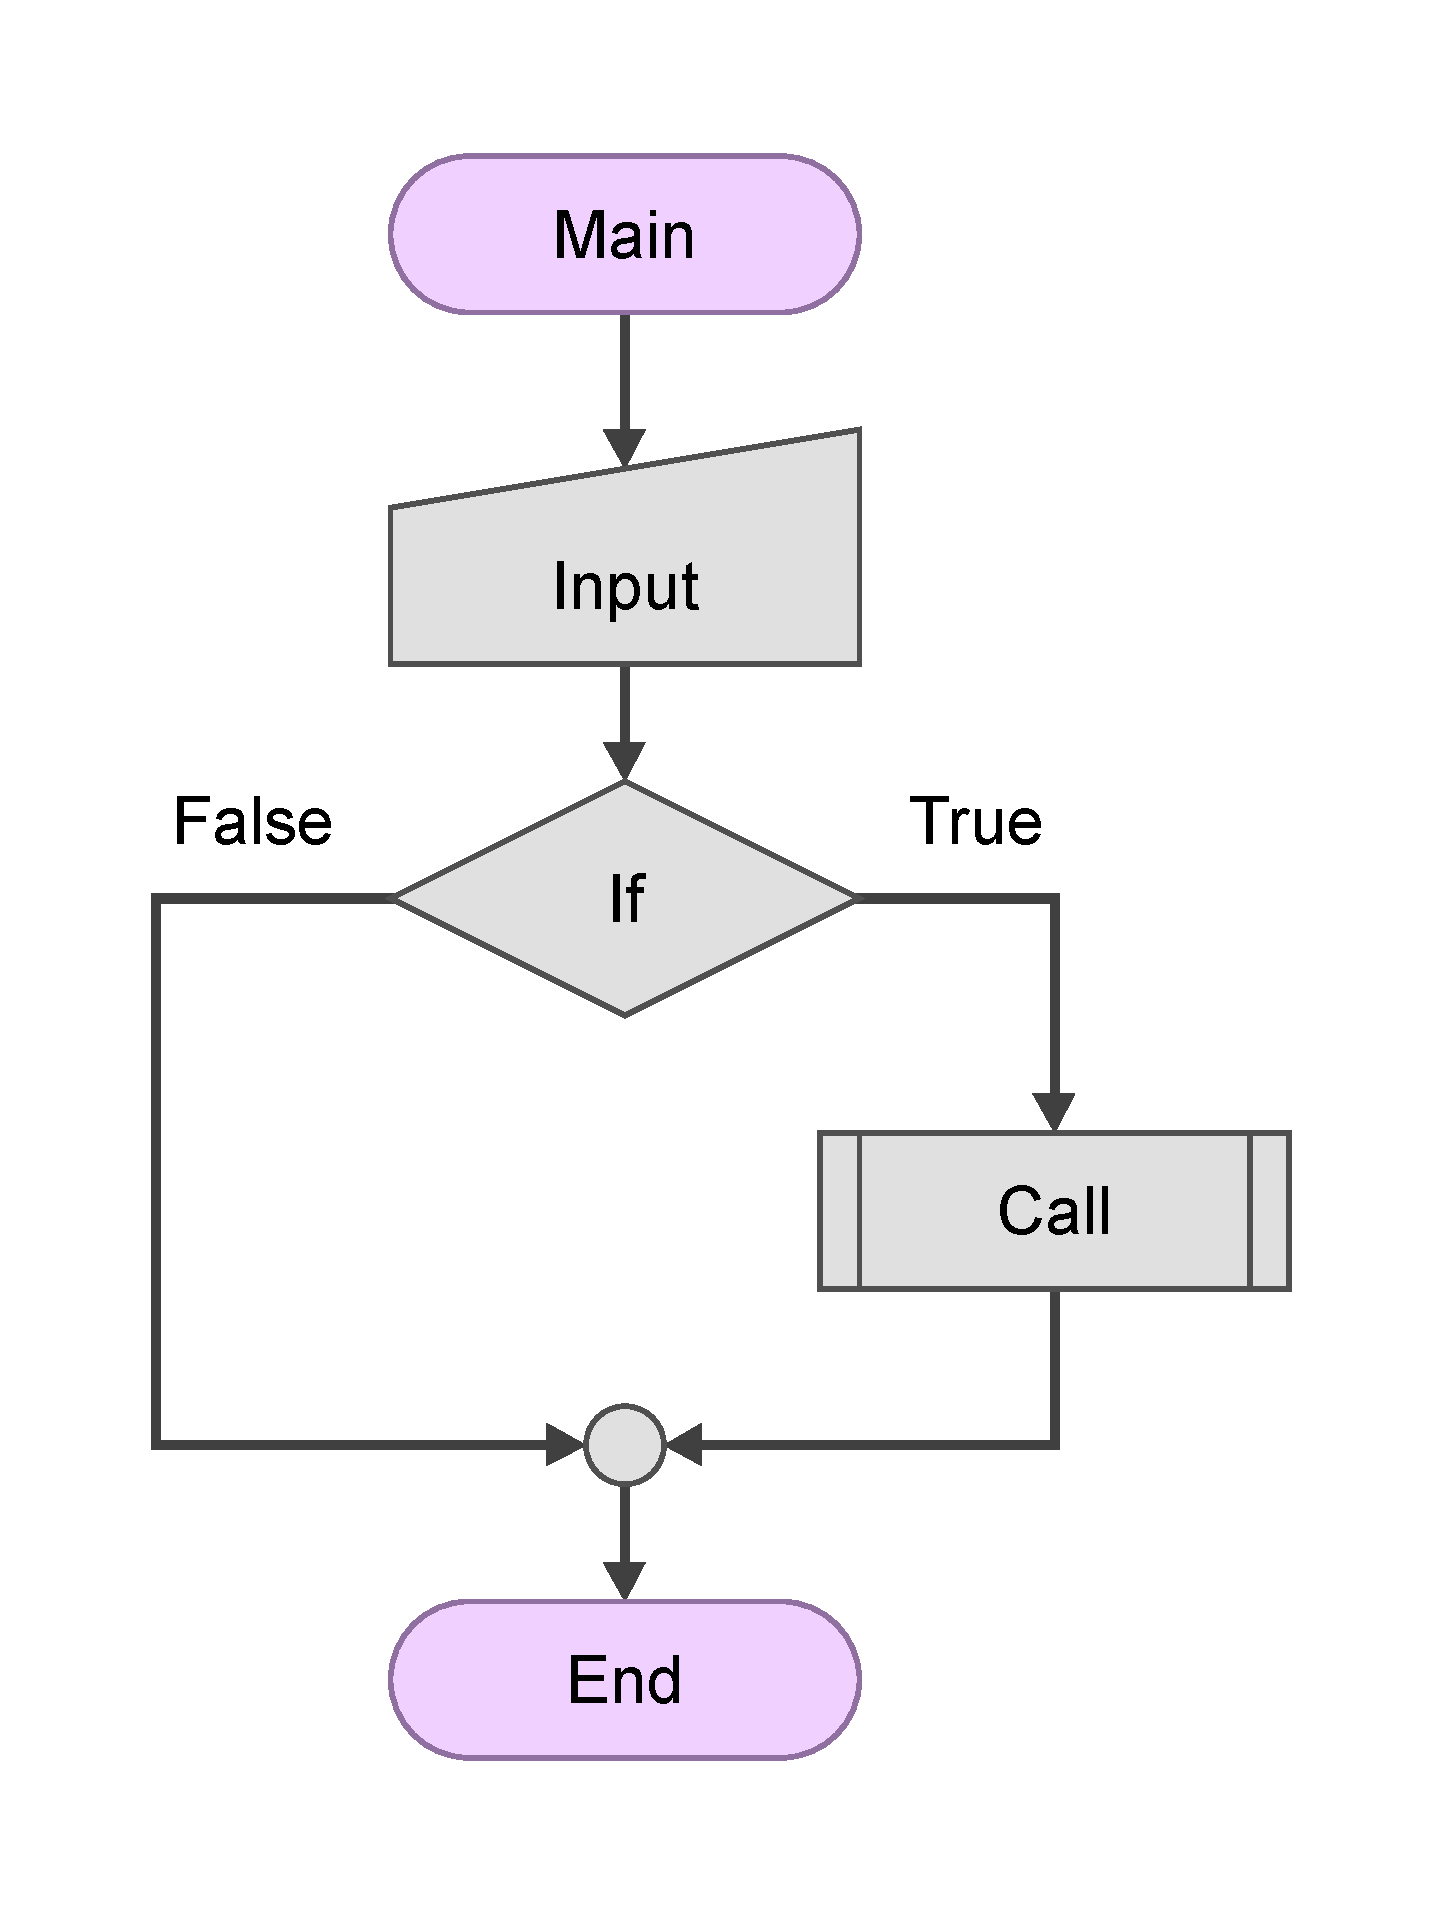
\includegraphics[scale=0.3]{figures/chart.pdf}
    \caption{Example figure in \LaTeX.}
    \label{fig:chart_a}
\end{figure}

\clearpage %  use command \clearpage when you want section or text to appear in the next page.

\section{Example of an algorithm in \LaTeX}
Algorithm~\ref{algo:algo_example} is a good example of an algorithm in \LaTeX.  
\begin{algorithm}
    \caption{Example caption: sum of all even numbers}
    \label{algo:algo_example}
    \begin{algorithmic}[1]
        \Require{$ \mathbf{x}  = x_1, x_2, \ldots, x_N$}
        \Ensure{$EvenSum$ (Sum of even numbers in $ \mathbf{x} $)}
        \Statex
        \Function{EvenSummation}{$\mathbf{x}$}
        \State {$EvenSum$ $\gets$ {$0$}}
        \State {$N$ $\gets$ {$length(\mathbf{x})$}}
        \For{$i \gets 1$ to $N$}                    
        \If{$ x_i\mod 2 == 0$}  \Comment check if a number is even?
        \State {$EvenSum$ $\gets$ {$EvenSum + x_i$}}
        \EndIf
        \EndFor
        \State \Return {$EvenSum$}
        \EndFunction
    \end{algorithmic}
\end{algorithm}
 
\section{Example of code snippet  in \LaTeX}

Code Listing~\ref{list:python_code_ex} is a good example of including a code snippet in a report. While using code snippets, take care of the following:
\begin{itemize}
    \item do not paste your entire code (implementation) or everything you have coded. Add code snippets only. 
    \item The algorithm shown in Algorithm~\ref{algo:algo_example} is usually preferred over code snippets in a technical/scientific report. 
    \item Make sure the entire code snippet or algorithm stays on a single page and does not overflow to another page(s).  
\end{itemize}

Here are three examples of code snippets for three different languages (Python, Java, and CPP) illustrated in Listings~\ref{list:python_code_ex}, \ref{list:java_code_ex}, and \ref{list:cpp_code_ex} respectively.  

\begin{lstlisting}[language=Python, caption={Code snippet in \LaTeX ~and  this is a Python code example}, label=list:python_code_ex]
import numpy as np

x  = [0, 1, 2, 3, 4, 5] # assign values to an array
evenSum = evenSummation(x) # call a function

def evenSummation(x):
    evenSum = 0
    n = len(x)
    for i in range(n):
        if np.mod(x[i],2) == 0: # check if a number is even?
            evenSum = evenSum + x[i]
    return evenSum
\end{lstlisting}

Here we used  the ``\textbackslash clearpage'' command and forced-out the second listing example onto the next page. 
\clearpage  %
\begin{lstlisting}[language=Java, caption={Code snippet in \LaTeX ~and  this is a Java code example}, label=list:java_code_ex]
public class EvenSum{ 
    public static int evenSummation(int[] x){
        int evenSum = 0;
        int n = x.length;
        for(int i = 0; i < n; i++){
            if(x[i]%2 == 0){ // check if a number is even?
                evenSum = evenSum + x[i];
            }
        }
        return evenSum;     
    }
    public static void main(String[] args){ 
        int[] x  = {0, 1, 2, 3, 4, 5}; // assign values to an array
        int evenSum = evenSummation(x);
        System.out.println(evenSum);
    } 
} 
\end{lstlisting}


\begin{lstlisting}[language=C, caption={Code snippet in \LaTeX ~and  this is a C/C++ code example}, label=list:cpp_code_ex]
int evenSummation(int x[]){
    int evenSum = 0;
    int n = sizeof(x);
    for(int i = 0; i < n; i++){
        if(x[i]%2 == 0){ // check if a number is even?
            evenSum = evenSum + x[i];
    	}
    }
    return evenSum;     
}

int main(){
    int x[]  = {0, 1, 2, 3, 4, 5}; // assign values to an array
    int evenSum = evenSummation(x);
    cout<<evenSum;
    return 0;
}
\end{lstlisting}



\section{Example of in-text citation style}
\subsection{Example of the equations and illustrations placement and reference in the text}
Make sure whenever you refer to the equations, tables, figures, algorithms,  and listings for the first time, they also appear (placed) somewhere on the same page or in the following page(s). Always make sure to refer to the equations, tables and figures used in the report. Do not leave them without an \textbf{in-text citation}. You can refer to equations, tables and figures more them once.

\subsection{Example of the equations and illustrations style}
Write \textbf{Eq.} with an uppercase ``Eq`` for an equation before using an equation number with (\textbackslash eqref\{.\}). Use ``Table'' to refer to a table, ``Figure'' to refer to a figure, ``Algorithm'' to refer to an algorithm and ``Listing'' to refer to listings (code snippets). Note that, we do not use the articles ``a,'' ``an,'' and ``the'' before the words Eq., Figure, Table, and Listing, but you may use an article for referring the words figure, table, etc. in general.

For example, the sentence ``A report structure is shown in \textbf{the} Table~\ref{tab:gen_template}'' should be written as ``A report structure is shown \textbf{in} Table~\ref{tab:gen_template}.'' 
 

\section{Summary}
Write a summary of this chapter.

~\\[5em]
\noindent
{\huge\textbf{Note:}} In the case of \textbf{software engineering} project a Chapter ``\textbf{Testing and Validation}'' should precede the ``Results'' chapter. See Section~\ref{subsec:se_chpters} for report organization of such project. 


    \chapter{Results}
\label{ch:results}
The results chapter tells a reader about your findings based on the methodology you have used to solve the investigated problem. For example: 
\begin{itemize}
    \item If your project aims to develop a software/web application, the results may be the developed software/system/performance of the system, etc., obtained using a relevant methodological approach in software engineering. 
    
    \item If your project aims to implement an algorithm for its analysis, the results may be the performance of the algorithm obtained using a relevant experiment design. 
    
    \item If your project aims to solve some problems/research questions over a collected dataset, the results may be the findings obtained using the applied tools/algorithms/etc. 
\end{itemize}
Arrange your results and findings in a logical sequence. 



\section{A section}

...

\clearpage
\section{Example of a Table in \LaTeX}
Table~\ref{tab:_ex_tab} is an example of a table created using the package \LaTeX  ``booktabs.'' do check the link: \href{https://en.wikibooks.org/wiki/LaTeX/Tables}{wikibooks.org/wiki/LaTeX/Tables} for more details. A table should be clean and readable. Unnecessary horizontal lines and vertical lines in tables make them unreadable and messy. The example in Table~\ref{tab:_ex_tab} uses a minimum number of liens (only necessary ones). Make sure that the top rule and bottom rule (top and bottom horizontal lines) of a table are present. 

\begin{table}[h!]
    \centering
    \caption{Example of a table in \LaTeX}
    \label{tab:_ex_tab}
    \begin{tabular}{llr}     
        \toprule
        \multicolumn{2}{c}{Bike} \\
        \cmidrule(r){1-2}
        Type    &  Color & Price (\pounds) \\
        \midrule
        Electric    & black   & 700   \\
        Hybrid      & blue    & 500   \\
        Road        & blue    & 300   \\
        Mountain    & red     & 300   \\
        Folding     & black   & 500   \\
        \bottomrule
    \end{tabular}
\end{table}

\section{Example of captions style}

\begin{itemize}
    \item The \textbf{caption of a Figure (artwork) goes below} the artwork (Figure/Graphics/illustration). See example artwork in Figure~\ref{fig:chart_a}. 
    \item  The \textbf{caption of a Table goes above} the table. See the example in Table~\ref{tab:_ex_tab}.
    \item  The \textbf{caption of an Algorithm goes above} the algorithm. See the example in Algorithm~\ref{algo:algo_example}.
    \item The \textbf{caption of a Listing goes below} the Listing  (Code snippet). See example listing in Listing~\ref{list:python_code_ex}. 
\end{itemize} 





\section{Summary}
Write a summary of this chapter.




    \chapter{Discussion and Analysis}
\label{ch:discussion}

This chapter delves into the insights drawn from the results presented in the previous chapter, evaluating the performance of ChatGPT in generating solutions for data structures and algorithms (DSA) problems across various topics and under different prompts. The discussion aims to interpret the significance of the findings, highlight key limitations, and suggest avenues for future research.

\section{Impact of Keywords in Prompts on Acceptance Rates}
The effectiveness of the prompts in guiding ChatGPT towards successful solutions is notably influenced by specific keywords. For instance, the inclusion of the word "efficient" in Prompts 4, 6, and 9 correlated with a higher number of accepted solutions, as shown in Table~\ref{tab:accepted_solutions_per_prompt}. This suggests that directing ChatGPT to focus on efficiency not only in code execution but also in resource utilization resonates well with the model's capabilities in optimizing solutions.

\section{Role Influence on Prompt Performance}
Analysis of the role-specified in each prompt reveals a significant impact on performance. Prompts that described the user as an "expert" or "software engineer" tended to perform better, implying that a higher expectation in the role description possibly aligns better with ChatGPT's training on professional and technical language. Conversely, prompts that positioned the user as a "junior programmer" or "student" saw slightly lower acceptance rates, suggesting a mismatch between the complexity of problems and the assumed knowledge base of the role.

\section{Topic-wise Acceptance Rates}
Figure~\ref{fig:topic_wise_acceptance} presents a comparison of provided versus calculated acceptance rates across various DSA topics. The provided rates represent the expected success rates based on historical data, while the calculated rates are derived from ChatGPT's performance across nine prompts.

\begin{figure}[H]
    \centering
    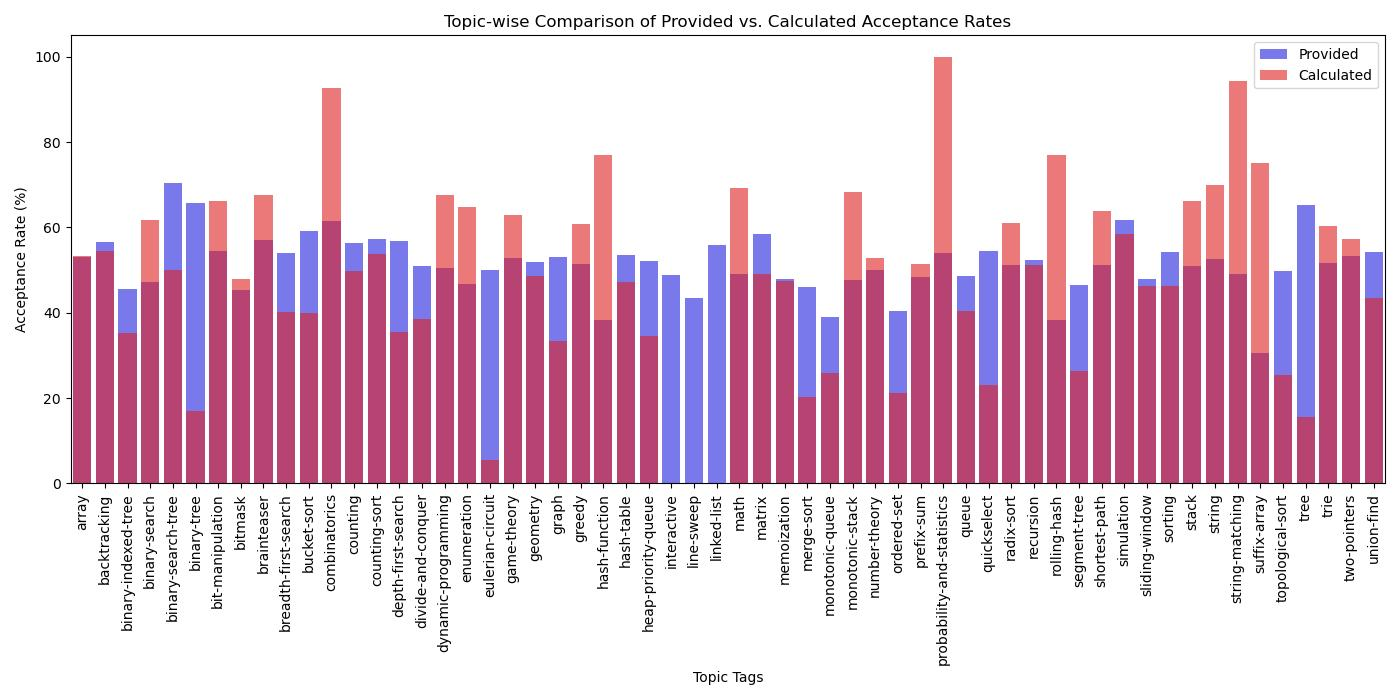
\includegraphics[width=1\textwidth]{figures/acceptance_topic_wise.jpg}
    \caption{Topic-wise comparison of provided vs. calculated acceptance rates}
    \label{fig:topic_wise_acceptance}
\end{figure}

ChatGPT exhibited exceptional performance in topics related to probability, statistics, combinatorics, hash function, rolling hash, string matching, and suffix array. These topics often involve a significant amount of mathematical reasoning and pattern recognition, areas where machine learning models like ChatGPT are particularly strong. On the other hand, the model struggled with topics such as binary tree, eulerian circuit, line sweep, linked list, and tree, which require a deep understanding of data structure manipulation and spatial relationships—a current limitation of language-based AI models.

\section{Implications of Findings}
The findings underscore the importance of prompt design in the effective utilization of AI for problem-solving in coding. By aligning the prompts with ChatGPT's training and capabilities, and by specifically targeting its strengths in mathematical reasoning and pattern recognition, the efficiency of AI-assisted coding solutions can be significantly enhanced.

\section{Limitations and Future Work}
While the study provides valuable insights into the capabilities of ChatGPT, it also highlights limitations, particularly in handling complex data structures. Future work could explore more granular prompt engineering, incorporate visual or spatial data representation techniques, and extend the analysis to newer versions of language models that might offer improved understanding of complex algorithms and data structures.

\section{Summary}
This chapter has discussed the key findings from the evaluation of ChatGPT's performance in solving DSA problems, highlighting how specific keywords and role expectations in prompts influence the effectiveness of the solutions generated. The analysis of topic-wise acceptance rates has revealed areas where ChatGPT excels and struggles, providing a roadmap for both leveraging its strengths and addressing its weaknesses in future applications.

    \chapter{Conclusions and Future Work}
\label{ch:con}
\section{Conclusions}
Typically a conclusions chapter first summarizes the investigated problem and its aims and objectives. It summaries the critical/significant/major findings/results about the aims and objectives that have been obtained by applying the key methods/implementations/experiment set-ups. A conclusions chapter draws a picture/outline of your project's central and the most signification contributions and achievements. 

A good conclusions summary could be approximately 300--500 words long, but this is just a recommendation.

A conclusions chapter followed by an abstract is the last things you write in your project report.

\section{Future work}
This section should refer to Chapter~\ref{ch:results} where the author has reflected their criticality about their own solution. The future work is then sensibly proposed in this section.

\textbf{Guidance on writing future work:} While working on a project, you gain experience and learn the potential of your project and its future works. Discuss the future work of the project in technical terms. This has to be based on what has not been yet achieved in comparison to what you had initially planned and what you have learned from the project. Describe to a reader what future work(s) can be started from the things you have completed. This includes identifying what has not been achieved and what could be achieved. 



A good future work summary could be approximately 300--500 words long, but this is just a recommendation.
    % \chapter{Reflection}
% \label{ch:reflection}
% %%%%%%%%%%%%%%%%%%%%%%%%%%%%%%%
% %% Please remove/replace text below
% %%%%%%%%%%%%%%%%%%%%%%%%%%%%%%%
% Write a short paragraph on the substantial learning experience. This can include your decision-making approach in problem-solving.

% \textbf{Some hints:} You obviously learned how to use different programming languages, write reports in \LaTeX and use other technical tools. In this section, we are more interested in what you thought about the experience. Take some time to think and reflect on your individual project as an experience, rather than just a list of technical skills and knowledge. You may describe things you have learned from the research approach and strategy, the process of identifying and solving a problem, the process research inquiry, and the understanding of the impact of the project on your learning experience and future work.

% Also think in terms of:
% \begin{itemize}
%     \item what knowledge and skills you have developed
%     \item what challenges you faced, but was not able to overcome
%     \item what you could do this project differently if the same or similar problem would come
%     \item rationalize the divisions from your initial planed aims and objectives.
% \end{itemize}


% A good reflective summary could be approximately 300--500 words long, but this is just a recommendation.

% ~\\[2em]
% \noindent
% {\huge \textbf{Note:}} The next chapter is ``\textbf{References},'' which will be automatically generated if you are using BibTeX referencing method. This template uses BibTeX referencing.  Also, note that there is difference between ``References'' and ``Bibliography.'' The list of ``References'' strictly only contain the list of articles, paper, and content you have cited (i.e., refereed) in the report. Whereas Bibliography is a list that contains the list of articles, paper, and content you have cited in the report plus the list of articles, paper, and content you have read in order to gain knowledge from. We recommend to use only the list of ``References.'' 
\chapter{Reflection}
\label{ch:reflection}

This project has been a profound journey into the capabilities and limitations of artificial intelligence, specifically within the context of solving data structures and algorithms (DSA) problems using ChatGPT. Reflecting on this experience, I recognize it as not only a technical exploration but also as a significant period of personal and professional growth.

One of the initial challenges I faced was the lack of libraries or open-source resources specifically tailored for gathering coding problems and their test cases. This limitation necessitated a deep dive into existing methodologies, which often fell short in directly addressing the needs of this project. The absence of a ready-made solution for fetching diverse and complex coding questions led me to develop a new approach for data acquisition. This process involved exploring various databases and APIs, eventually leading to the creation of an automated pipeline that utilized the LeetCode GraphQL API. This experience was invaluable as it pushed me to innovate and create tools that were not only useful for this project but also adaptable for future research in this field.

Throughout this project, I learned the critical importance of role-based prompt engineering. By crafting prompts that simulated different user roles—from a junior programmer to an expert in Python programming—I was able to significantly influence ChatGPT's output. This exploration revealed how subtle changes in language and the inclusion of specific keywords could dramatically alter the effectiveness of the solutions provided by the AI. The experience has sharpened my skills in understanding how to guide AI to perform tasks that it might not inherently excel at, especially in areas requiring a deep understanding of complex data structures.

A substantial portion of my time was devoted to analyzing the responses generated by ChatGPT, identifying patterns, and fine-tuning the post-processing of these solutions to ensure they could be executed on test cases without human intervention. This aspect of the project was particularly challenging due to the variability in the AI's responses. Developing a methodical approach to automatically adjust and correct the generated code was both challenging and rewarding. It underscored the importance of iterative testing and adjustment in AI-related projects, where outcomes can be unpredictable and require continuous refinement.

Looking back, if I were to tackle a similar problem in the future, I would place a greater emphasis on developing even more robust tools for data handling and analysis from the outset. The iterative nature of AI testing and the variability in model performance highlighted the need for flexible and adaptable project planning. 

Moreover, this project has significantly impacted my understanding of the role of AI in educational and professional settings. It has provided me with a solid foundation in research methodology, enhanced my problem-solving skills, and deepened my appreciation for the detailed and careful design required to successfully implement AI solutions. The insights gained from this project will undoubtedly influence my approach to future AI research and applications, particularly in optimizing the interaction between human input and AI output.

Overall, this reflective summary encapsulates not just a list of technical skills acquired but also the broader learning experiences—highlighting challenges, adaptations, and personal insights gained throughout the duration of the project.

    

    
    % -------------------------------------------------------------------
    % Bibliography/References  -  Harvard Style was used in this report
    % -------------------------------------------------------------------
    \bibliographystyle{agsm} % Harvard Style 
    
    \bibliography{references}  %  Patashnik, O. (1988), BibTEXing. Documentation for general BibTEX users.
    
    % -------------------------------------------------------------------
    % Appendices
    % -------------------------------------------------------------------
    
    \begin{appendices}
        \chapter{An Appendix Chapter}
\label{appn:A}

\section{Topic-Wise Acceptance Rates for Each Prompt}
This section presents the topic-wise acceptance rates for each of the nine prompts used in the study. These figures illustrate how the model performed across various computer science topics, highlighting areas of strength and weakness for each prompt. These visualizations serve as a valuable tool for understanding the specific strengths and weaknesses of the AI model in solving diverse coding problems, and it can guide future research and prompt engineering efforts to enhance model performance.

\begin{figure}[H]
    \centering
    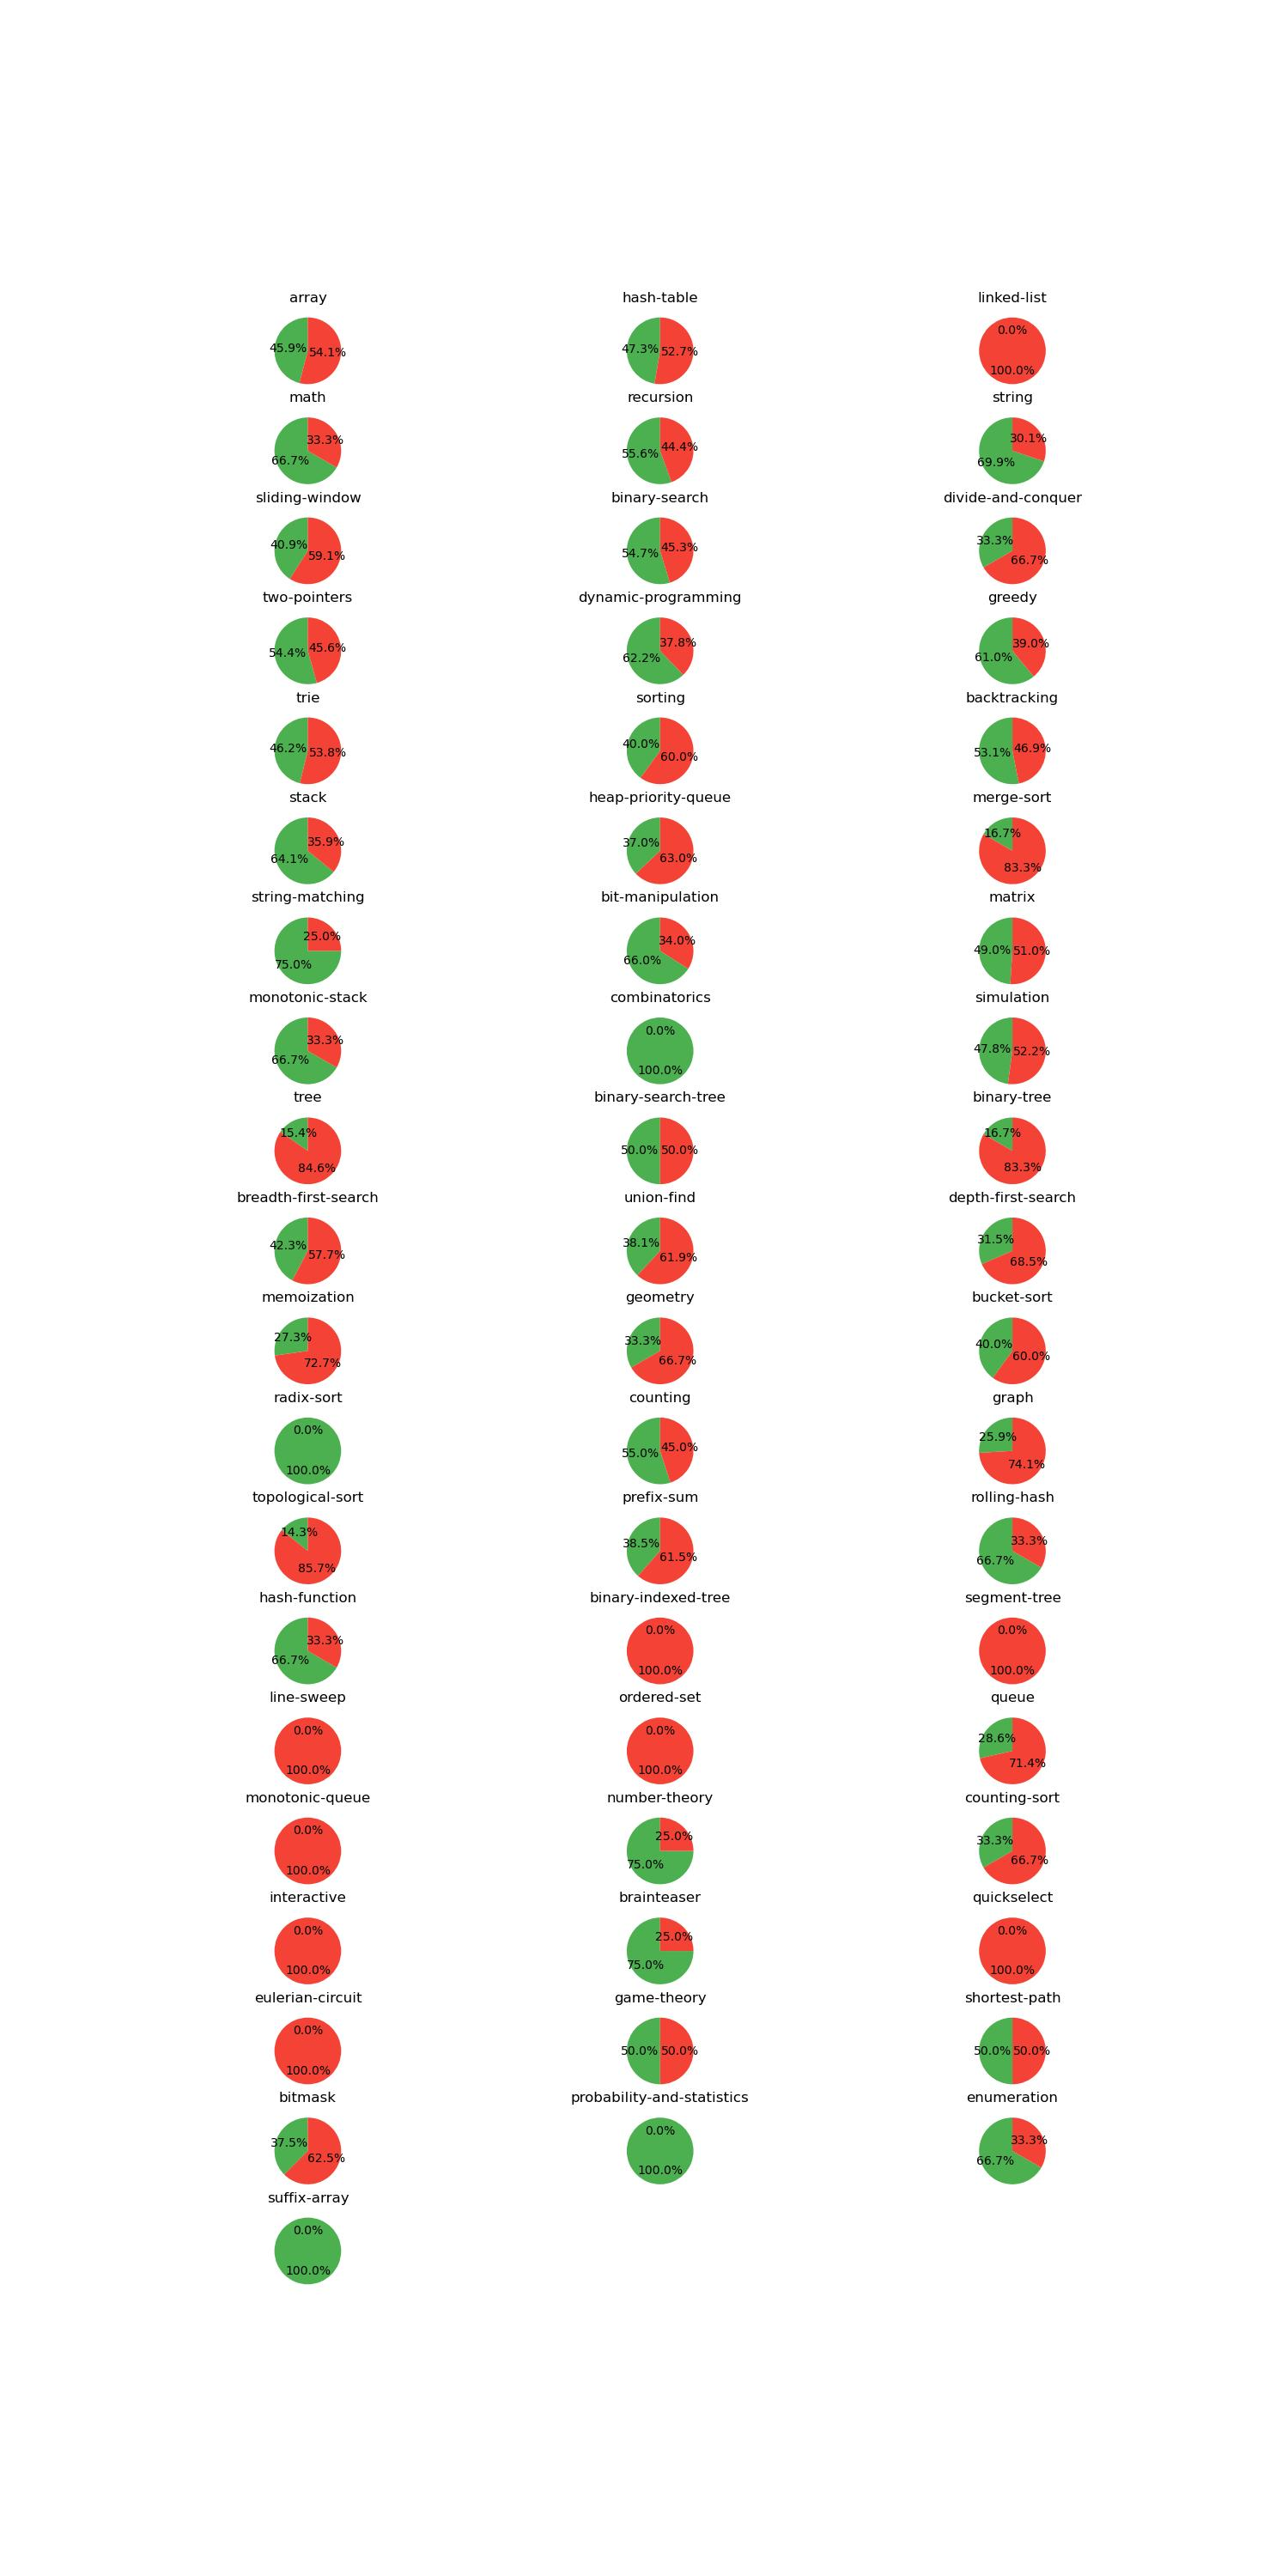
\includegraphics[width=0.75\textwidth, height=0.7\textheight]{figures/1/accepted_not_topicwise.jpg}
    \caption{Topic-wise acceptance rate for Prompt 1, illustrating the percentage of solutions accepted (green) and not accepted (red) across different undergraduate computer science topics.}
    \label{fig:topic_wise_acceptance_prompt_1}
\end{figure}

\begin{figure}[H]
    \centering
    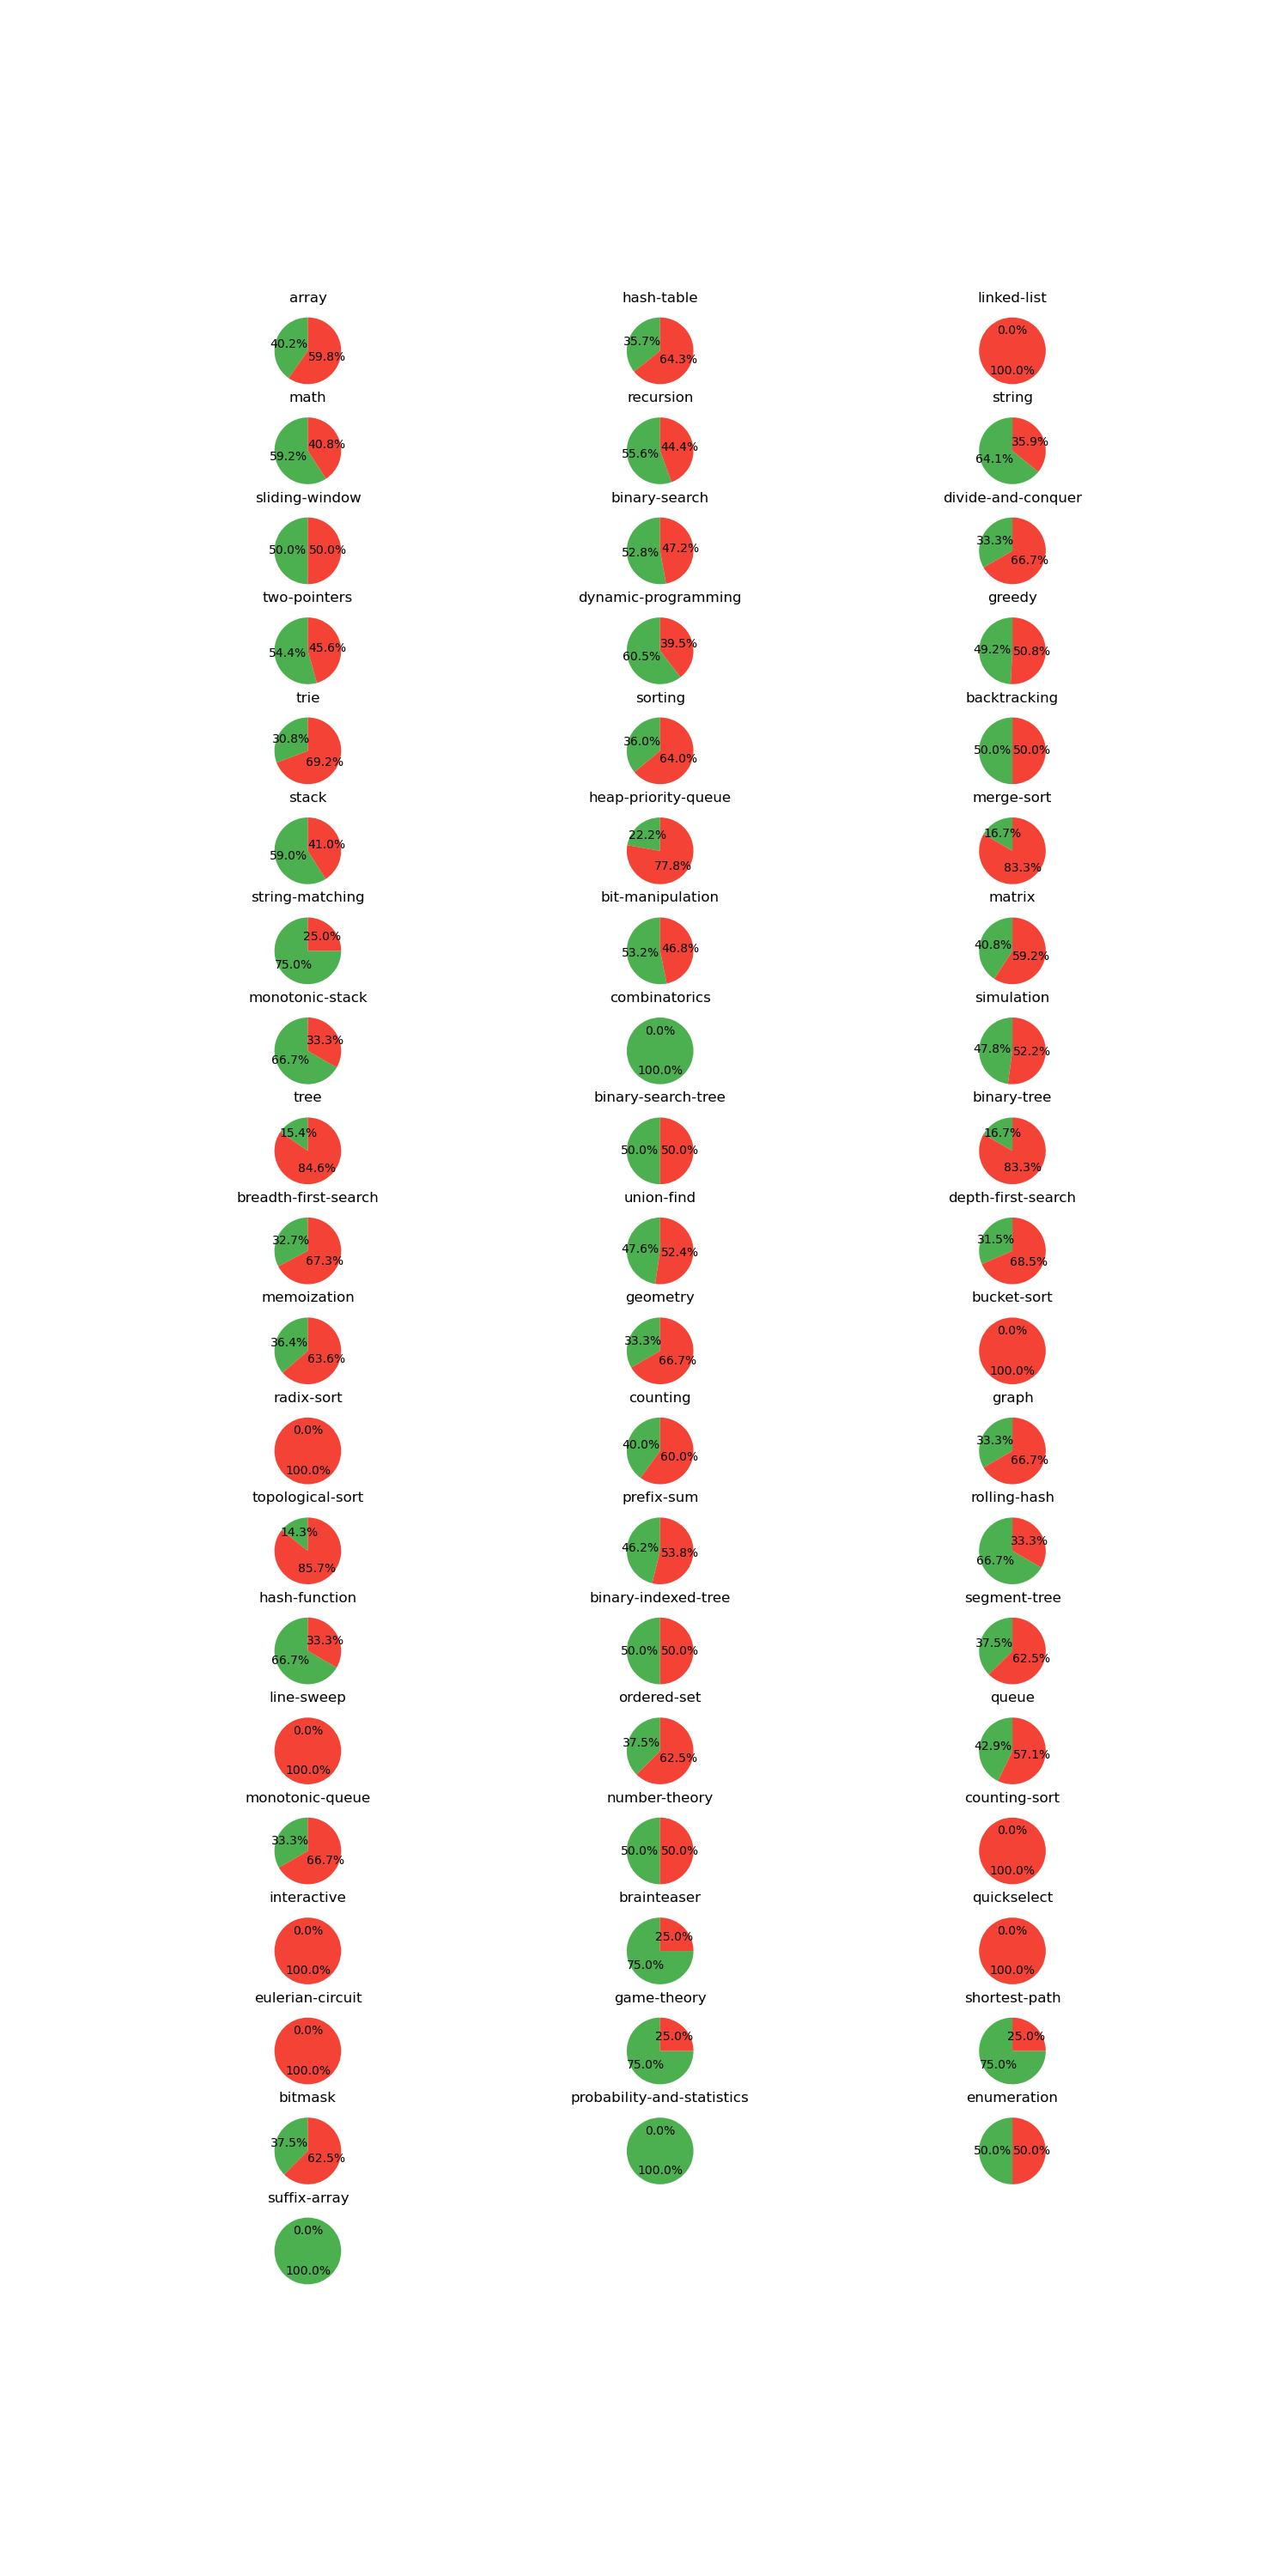
\includegraphics[width=0.75\textwidth, height=0.7\textheight]{figures/2/accepted_not_topicwise.jpg}
    \caption{Topic-wise acceptance rate for Prompt 2, illustrating the percentage of solutions accepted (green) and not accepted (red) across different undergraduate computer science topics.}
    \label{fig:topic_wise_acceptance_prompt_2}
\end{figure}

\begin{figure}[H]
    \centering
    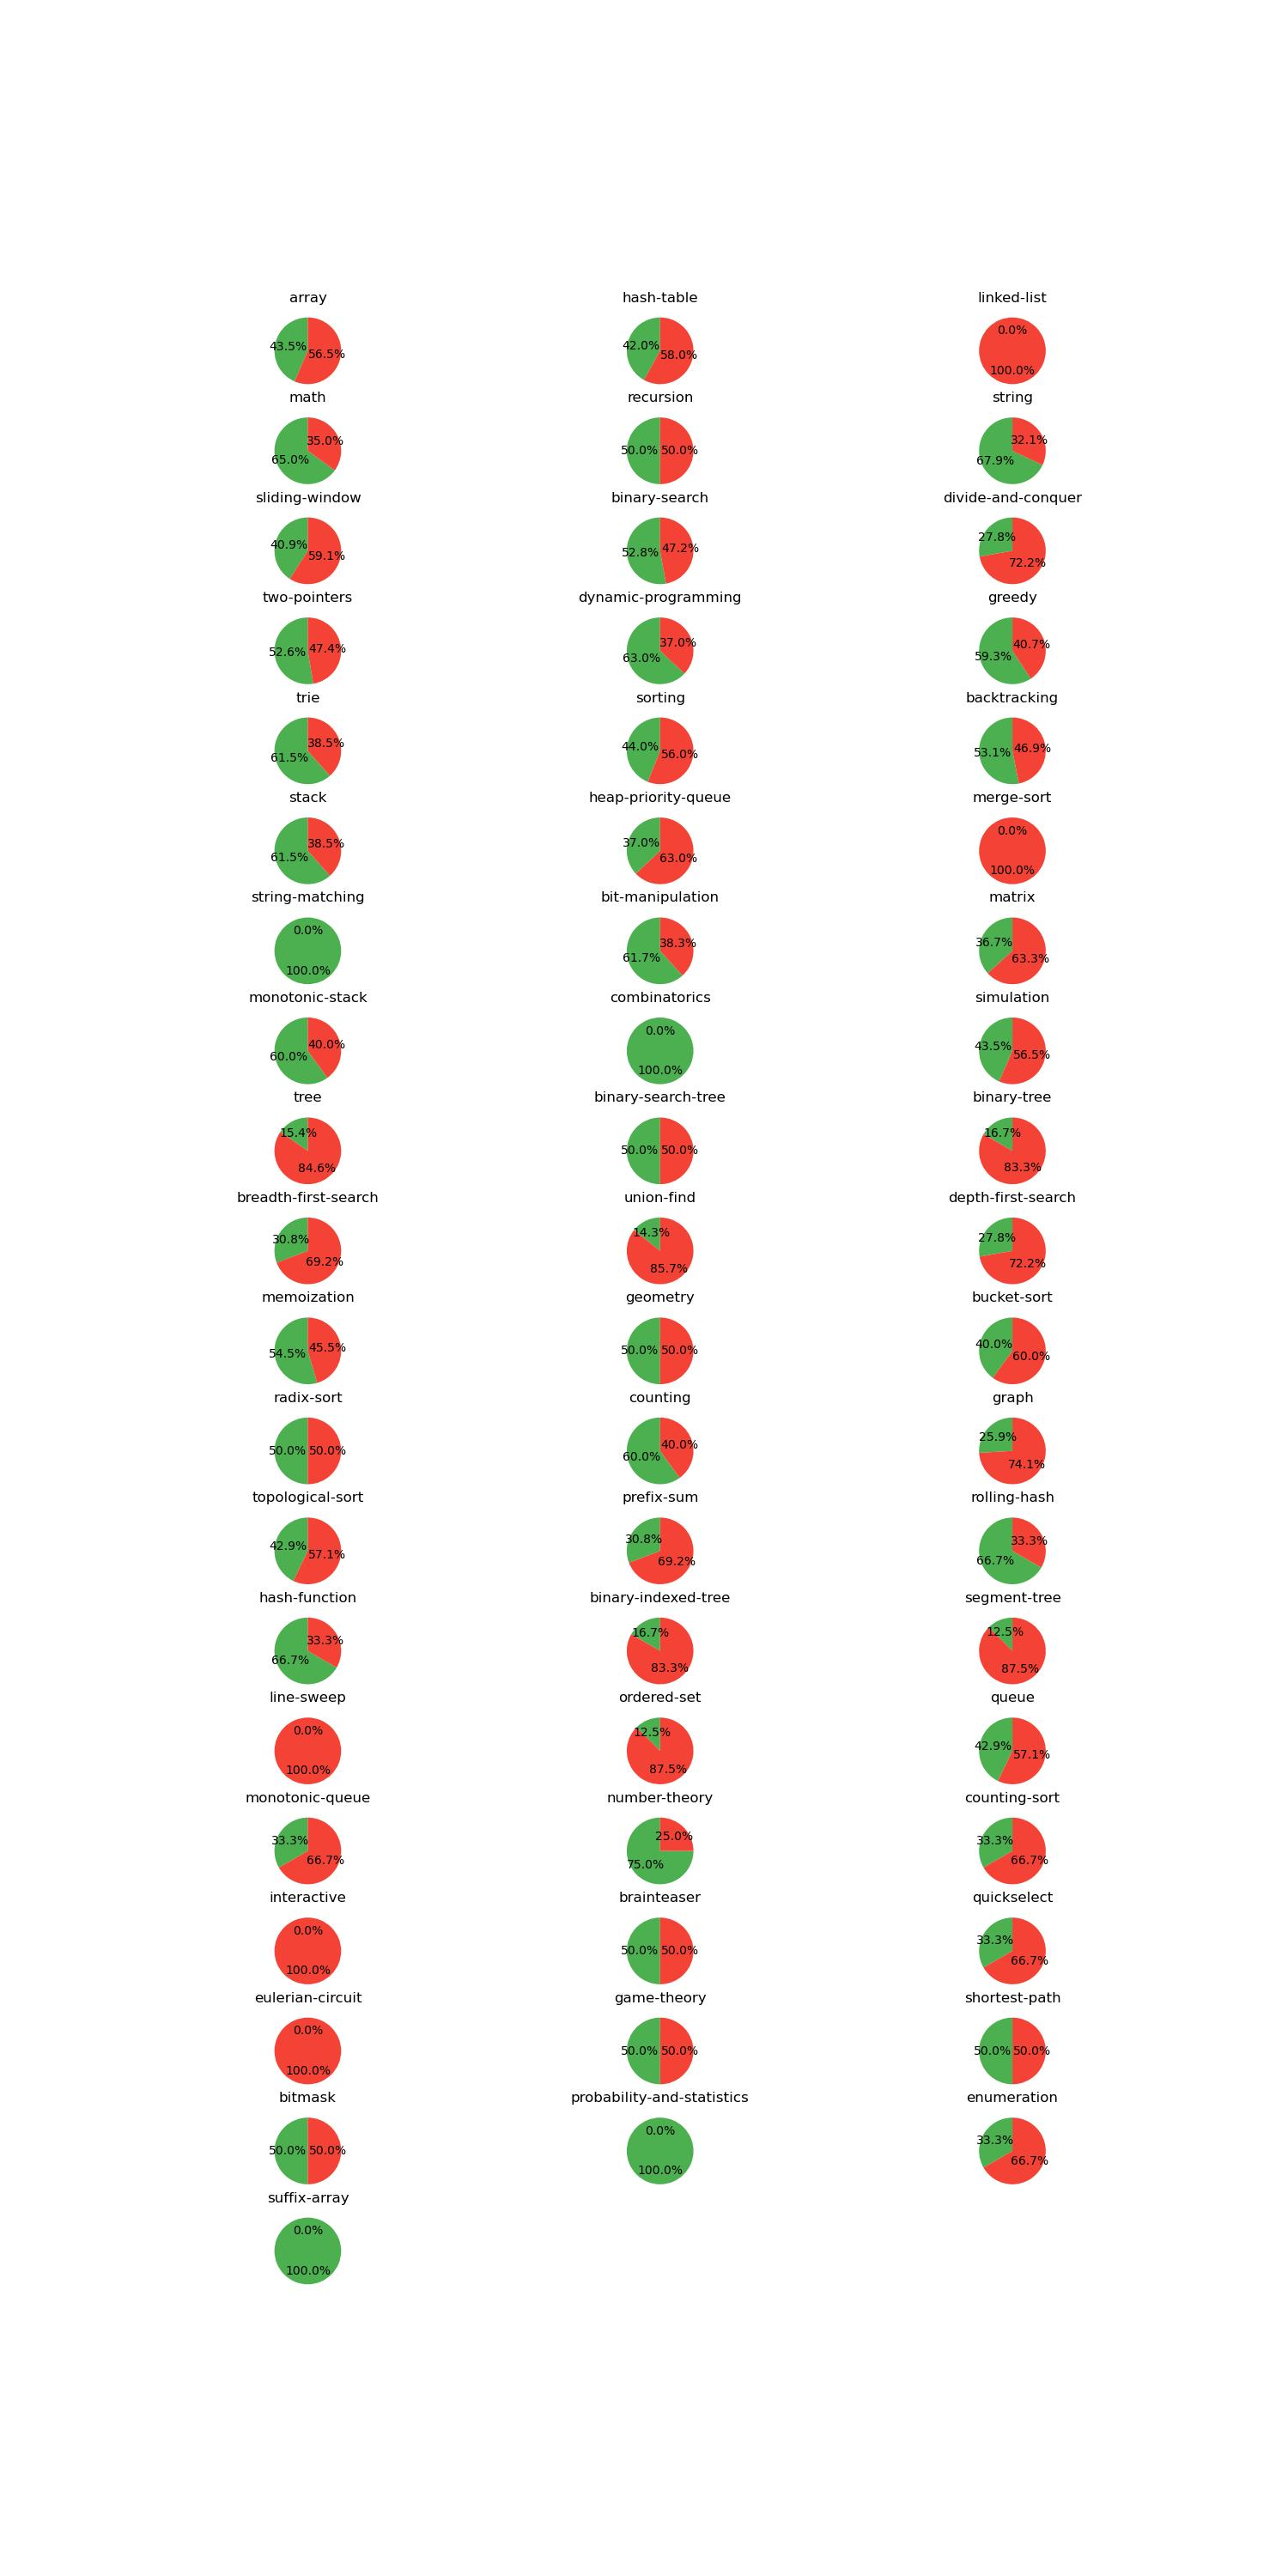
\includegraphics[width=0.75\textwidth, height=0.7\textheight]{figures/3/accepted_not_topicwise.jpg}
    \caption{Topic-wise acceptance rate for Prompt 3, illustrating the percentage of solutions accepted (green) and not accepted (red) across different undergraduate computer science topics.}
    \label{fig:topic_wise_acceptance_prompt_3}
\end{figure}

\begin{figure}[H]
    \centering
    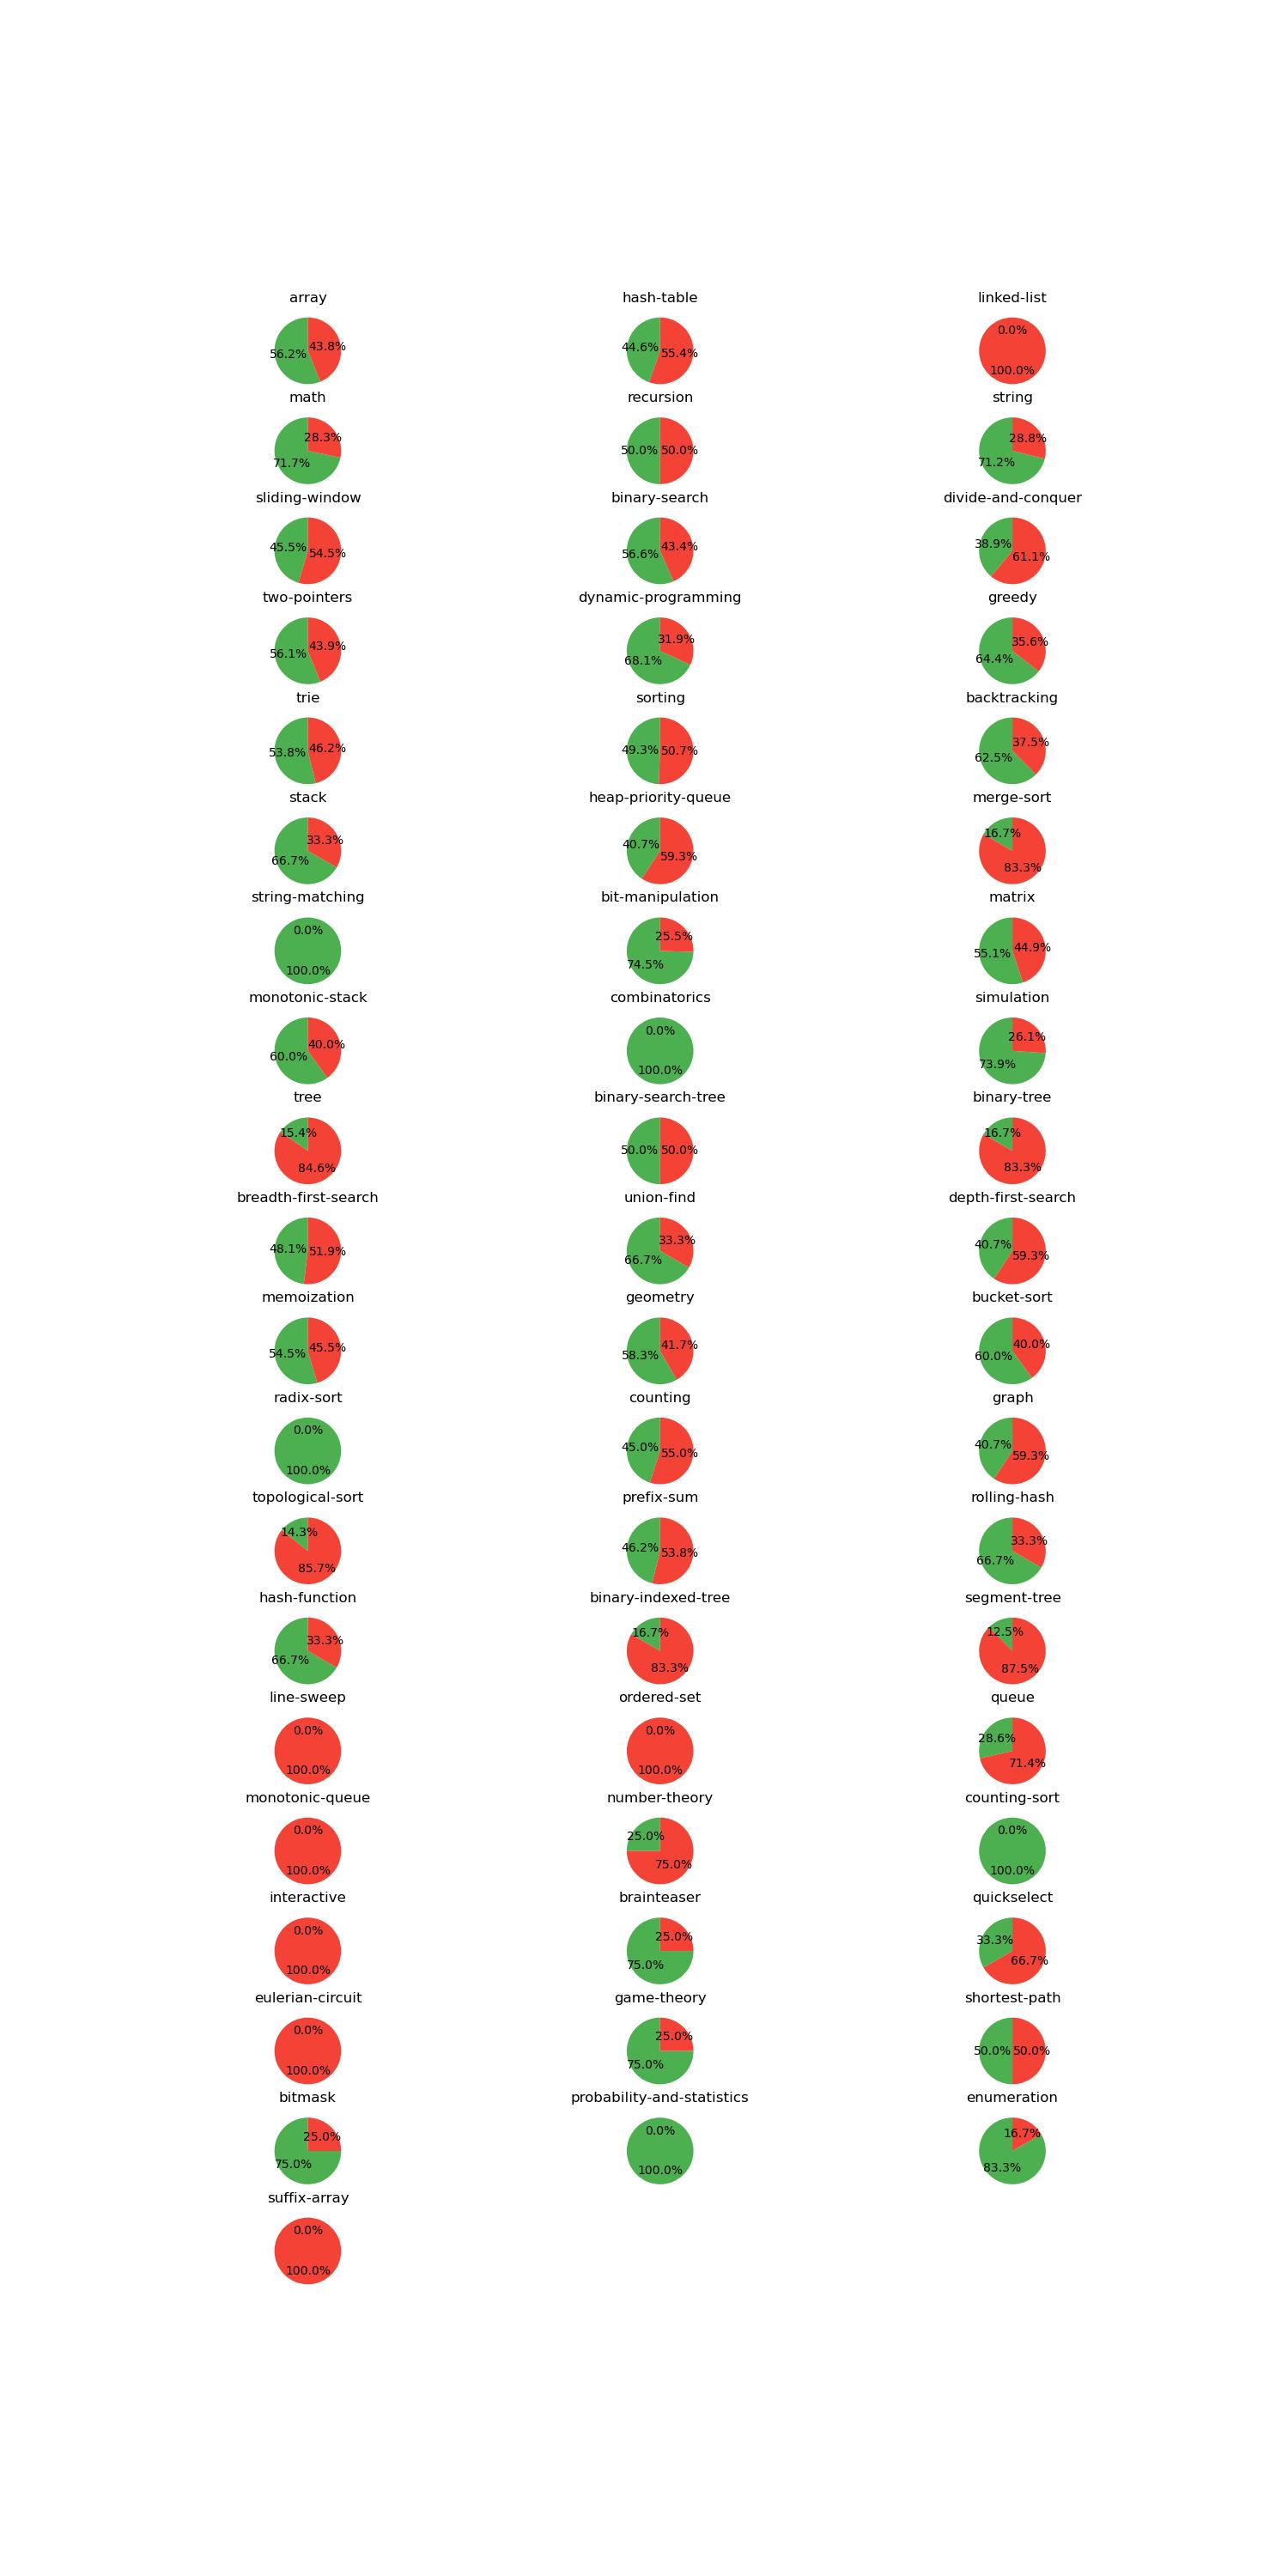
\includegraphics[width=0.75\textwidth, height=0.7\textheight]{figures/4/accepted_not_topicwise.jpg}
    \caption{Topic-wise acceptance rate for Prompt 4, illustrating the percentage of solutions accepted (green) and not accepted (red) across different undergraduate computer science topics.}
    \label{fig:topic_wise_acceptance_prompt_4}
\end{figure}

\begin{figure}[H]
    \centering
    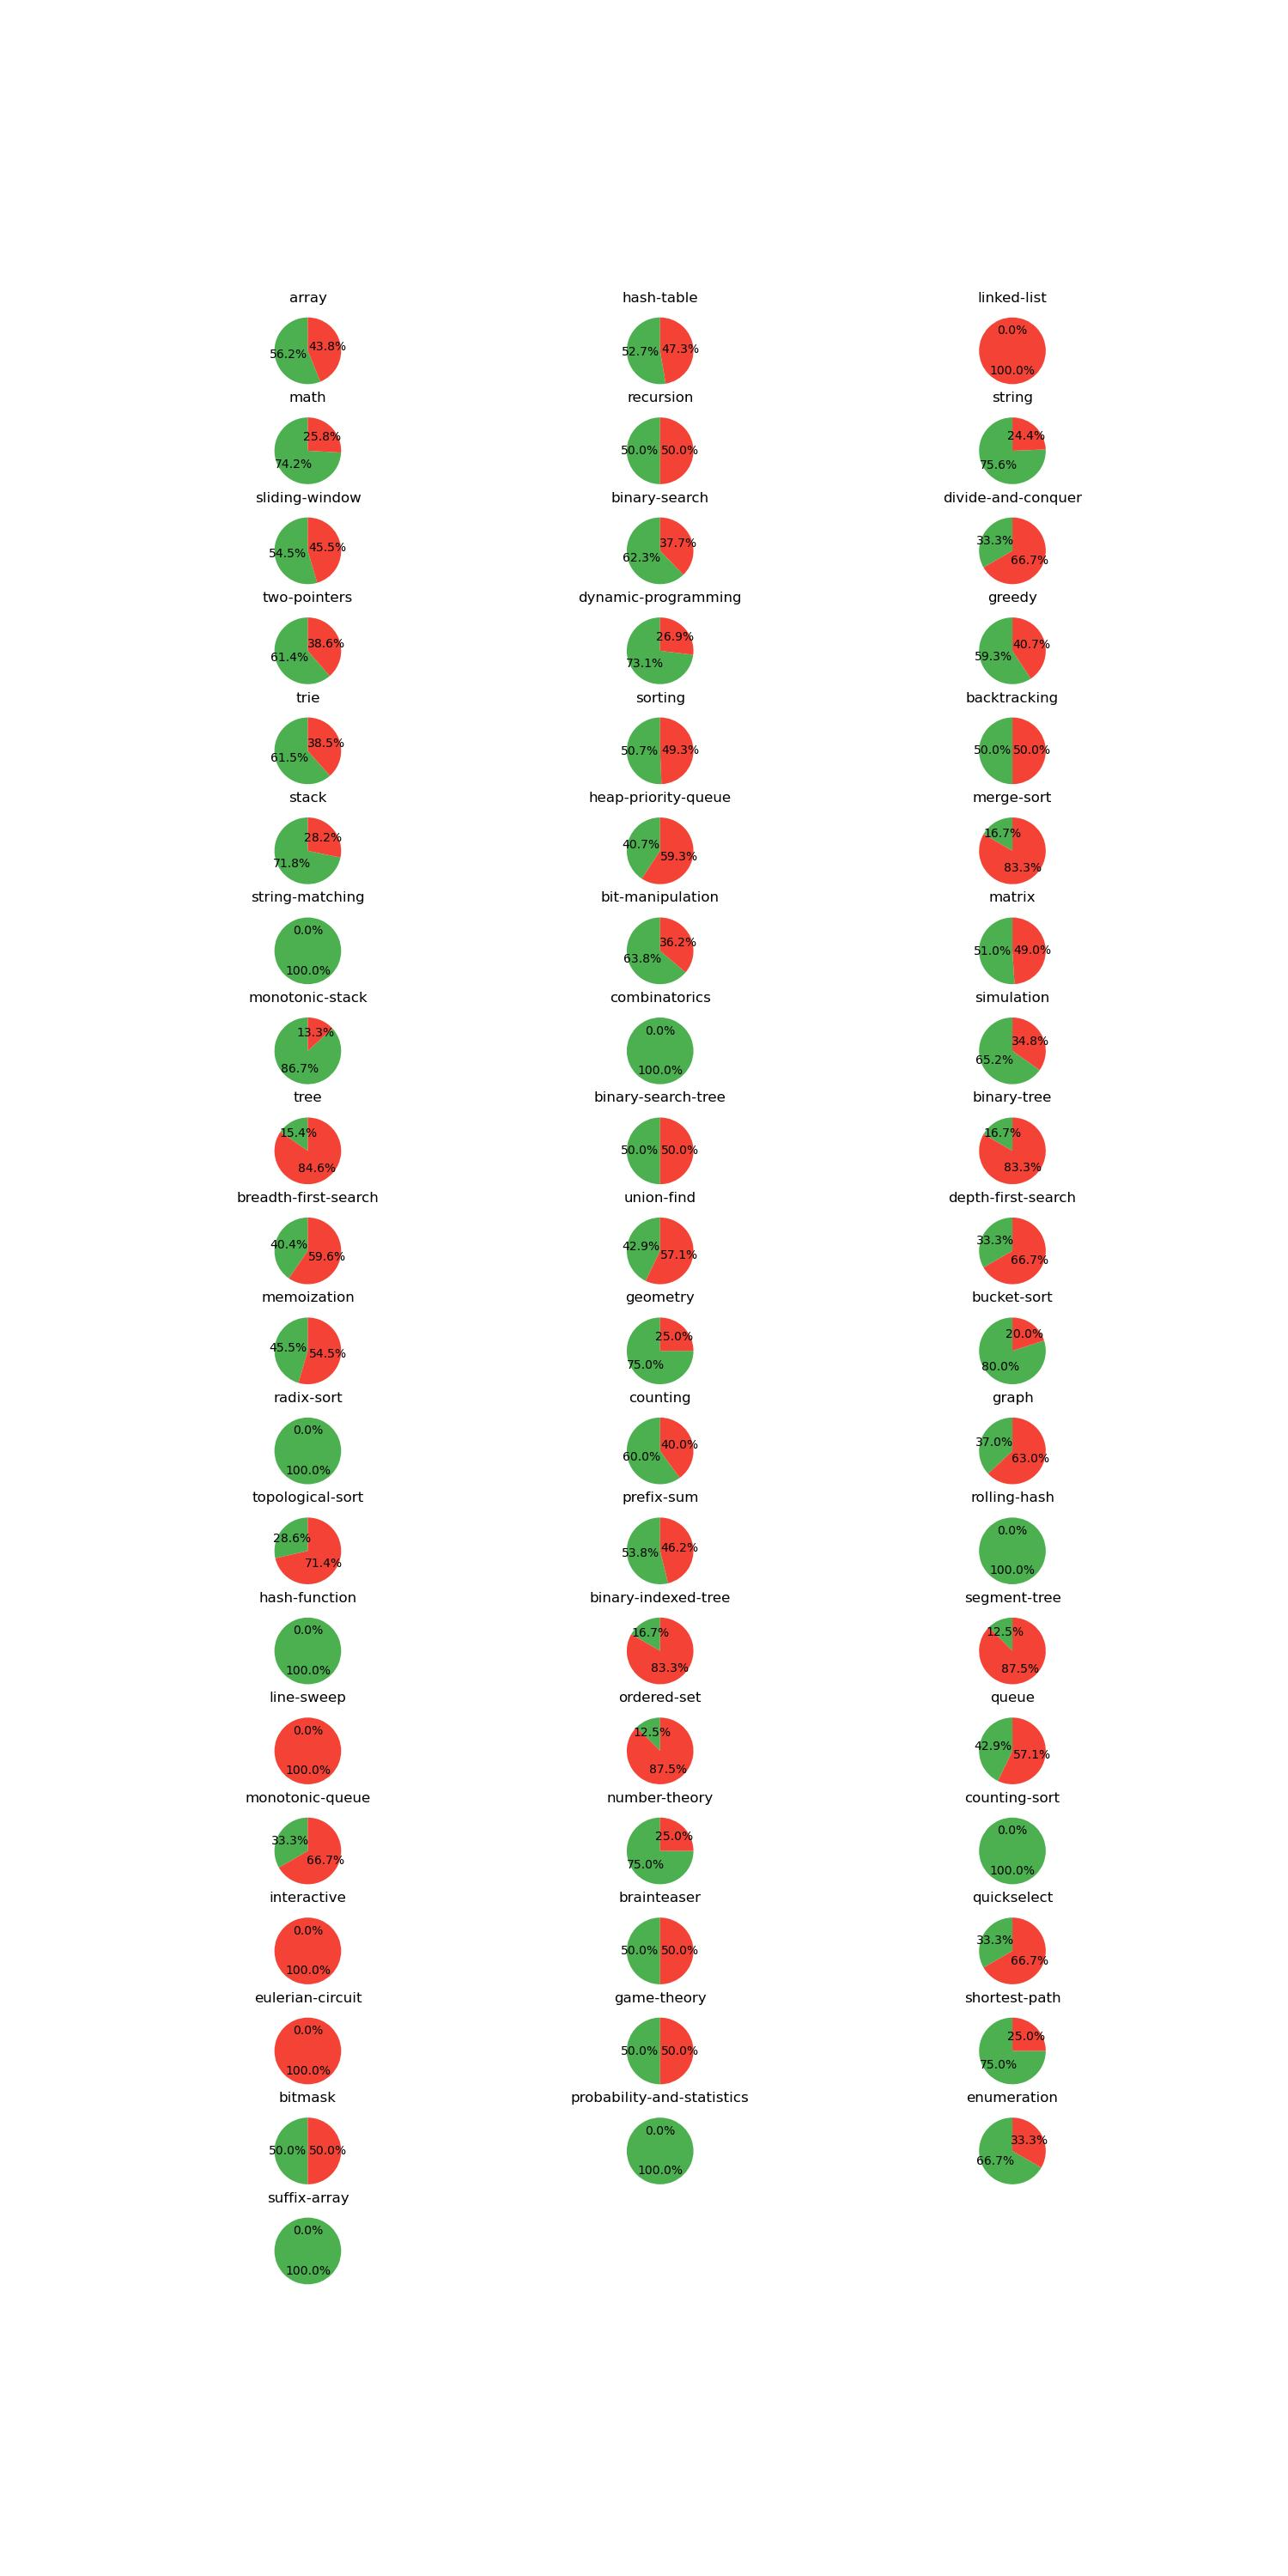
\includegraphics[width=0.75\textwidth, height=0.7\textheight]{figures/5/accepted_not_topicwise.jpg}
    \caption{Topic-wise acceptance rate for Prompt 5, illustrating the percentage of solutions accepted (green) and not accepted (red) across different undergraduate computer science topics.}
    \label{fig:topic_wise_acceptance_prompt_5}
\end{figure}

\begin{figure}[H]
    \centering
    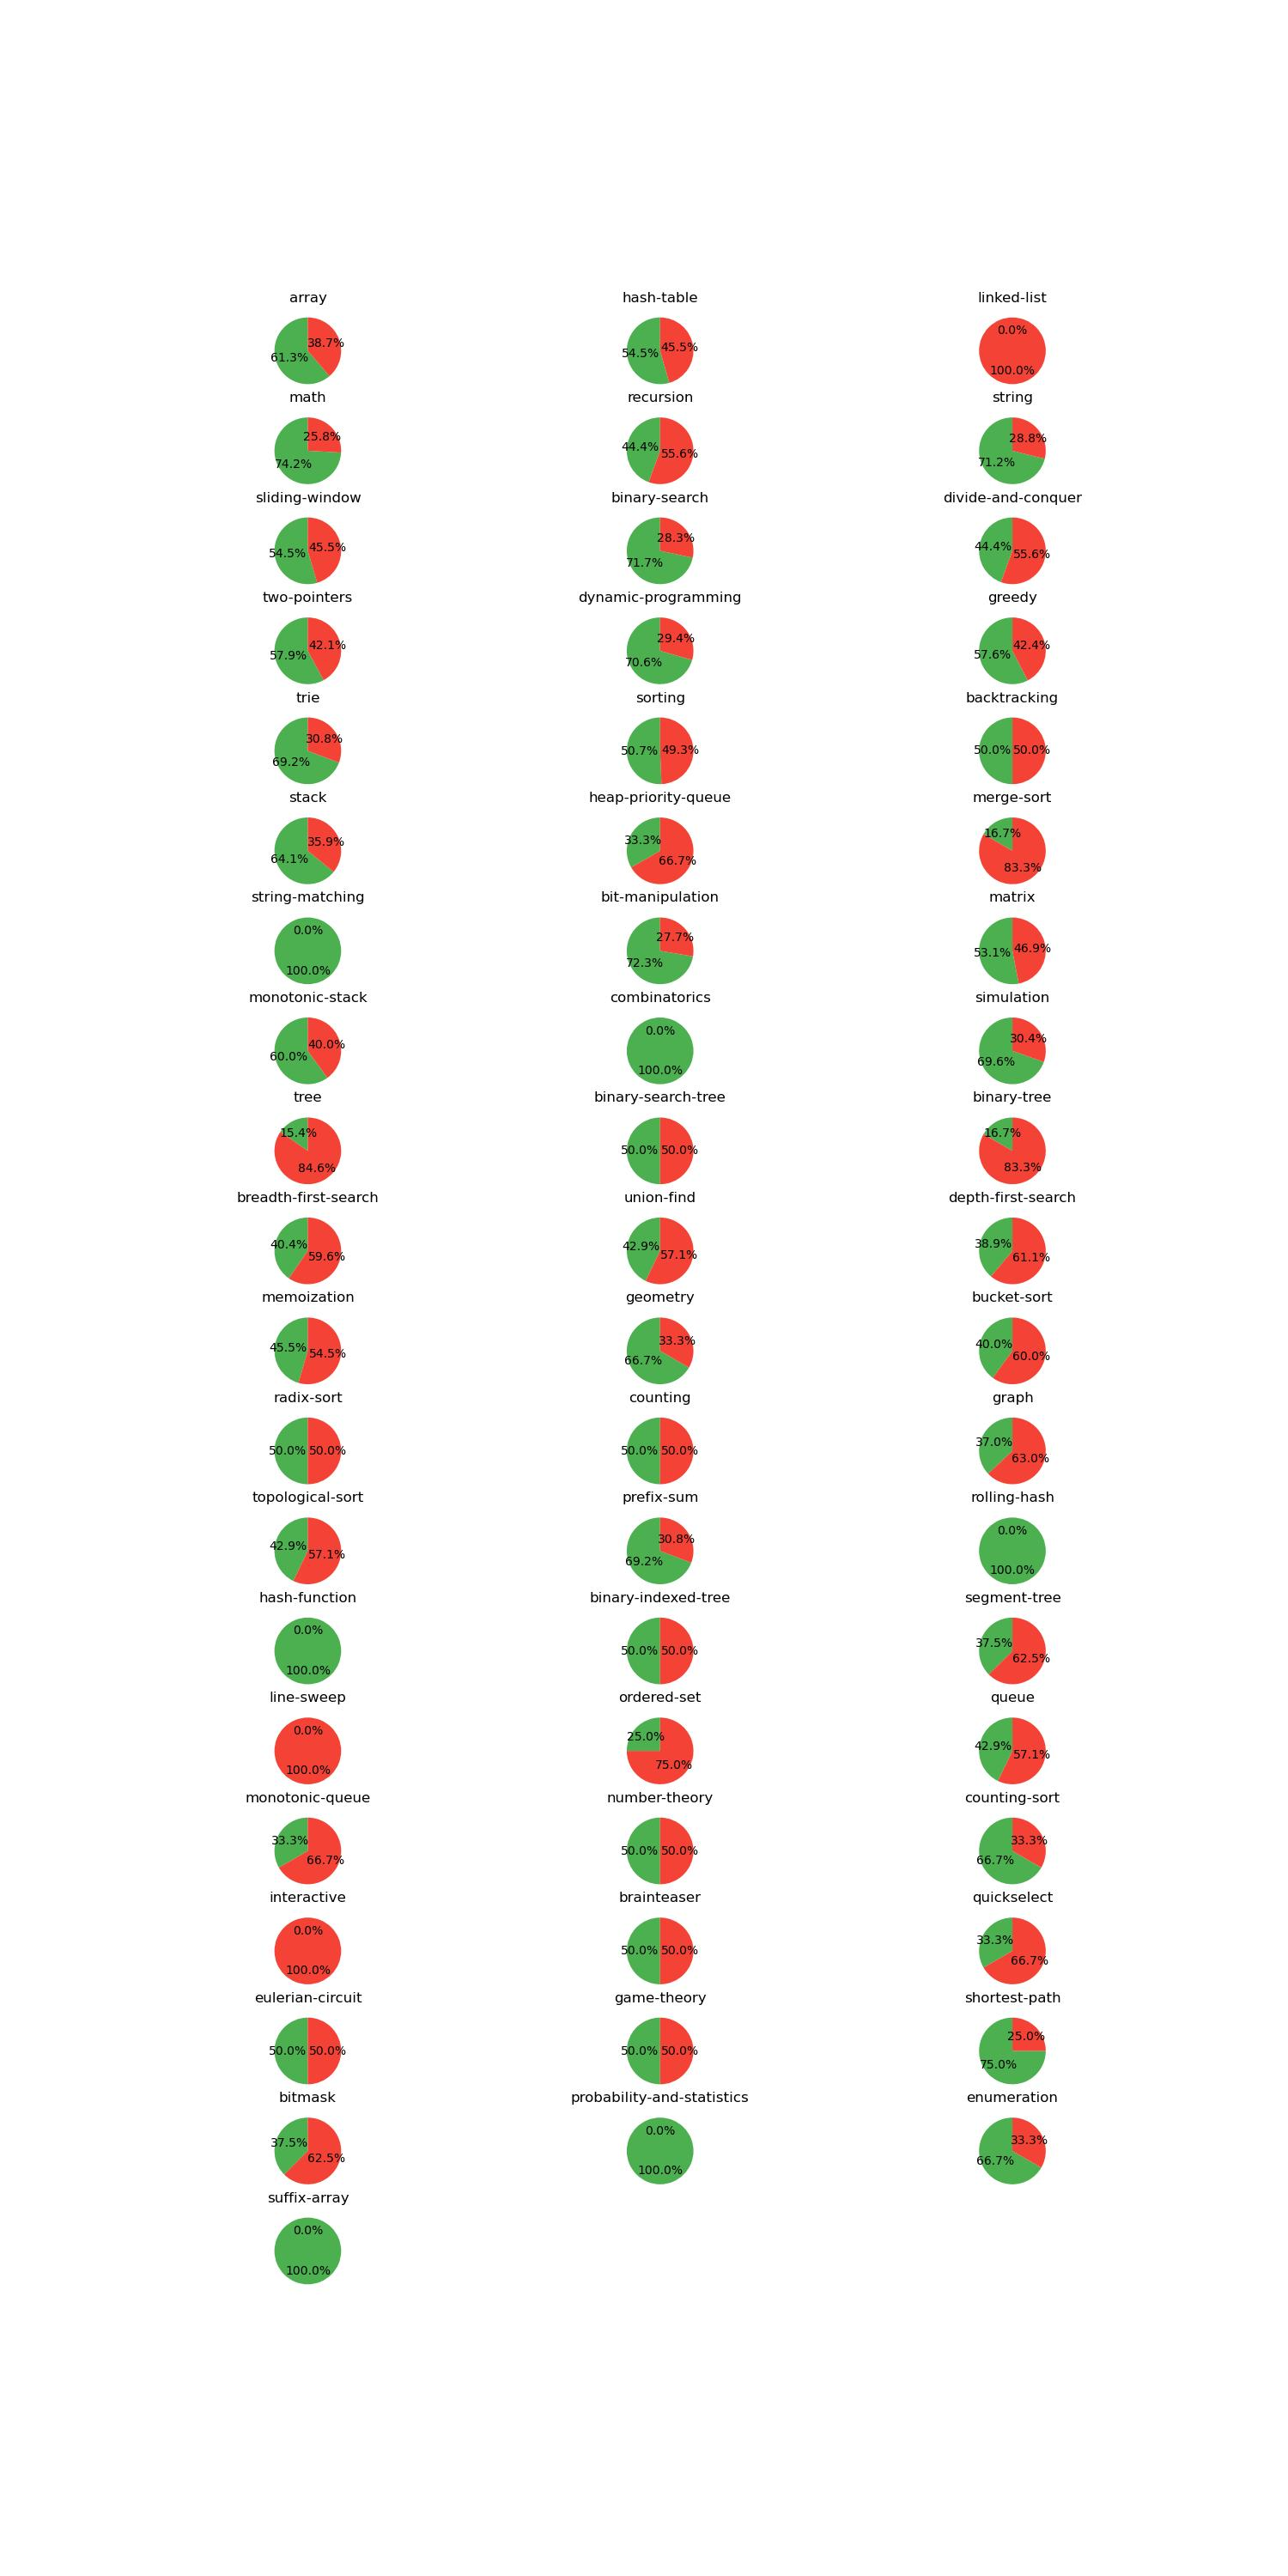
\includegraphics[width=0.75\textwidth, height=0.7\textheight]{figures/6/accepted_not_topicwise.jpg}
    \caption{Topic-wise acceptance rate for Prompt 6, illustrating the percentage of solutions accepted (green) and not accepted (red) across different undergraduate computer science topics.}
    \label{fig:topic_wise_acceptance_prompt_6}
\end{figure}

\begin{figure}[H]
    \centering
    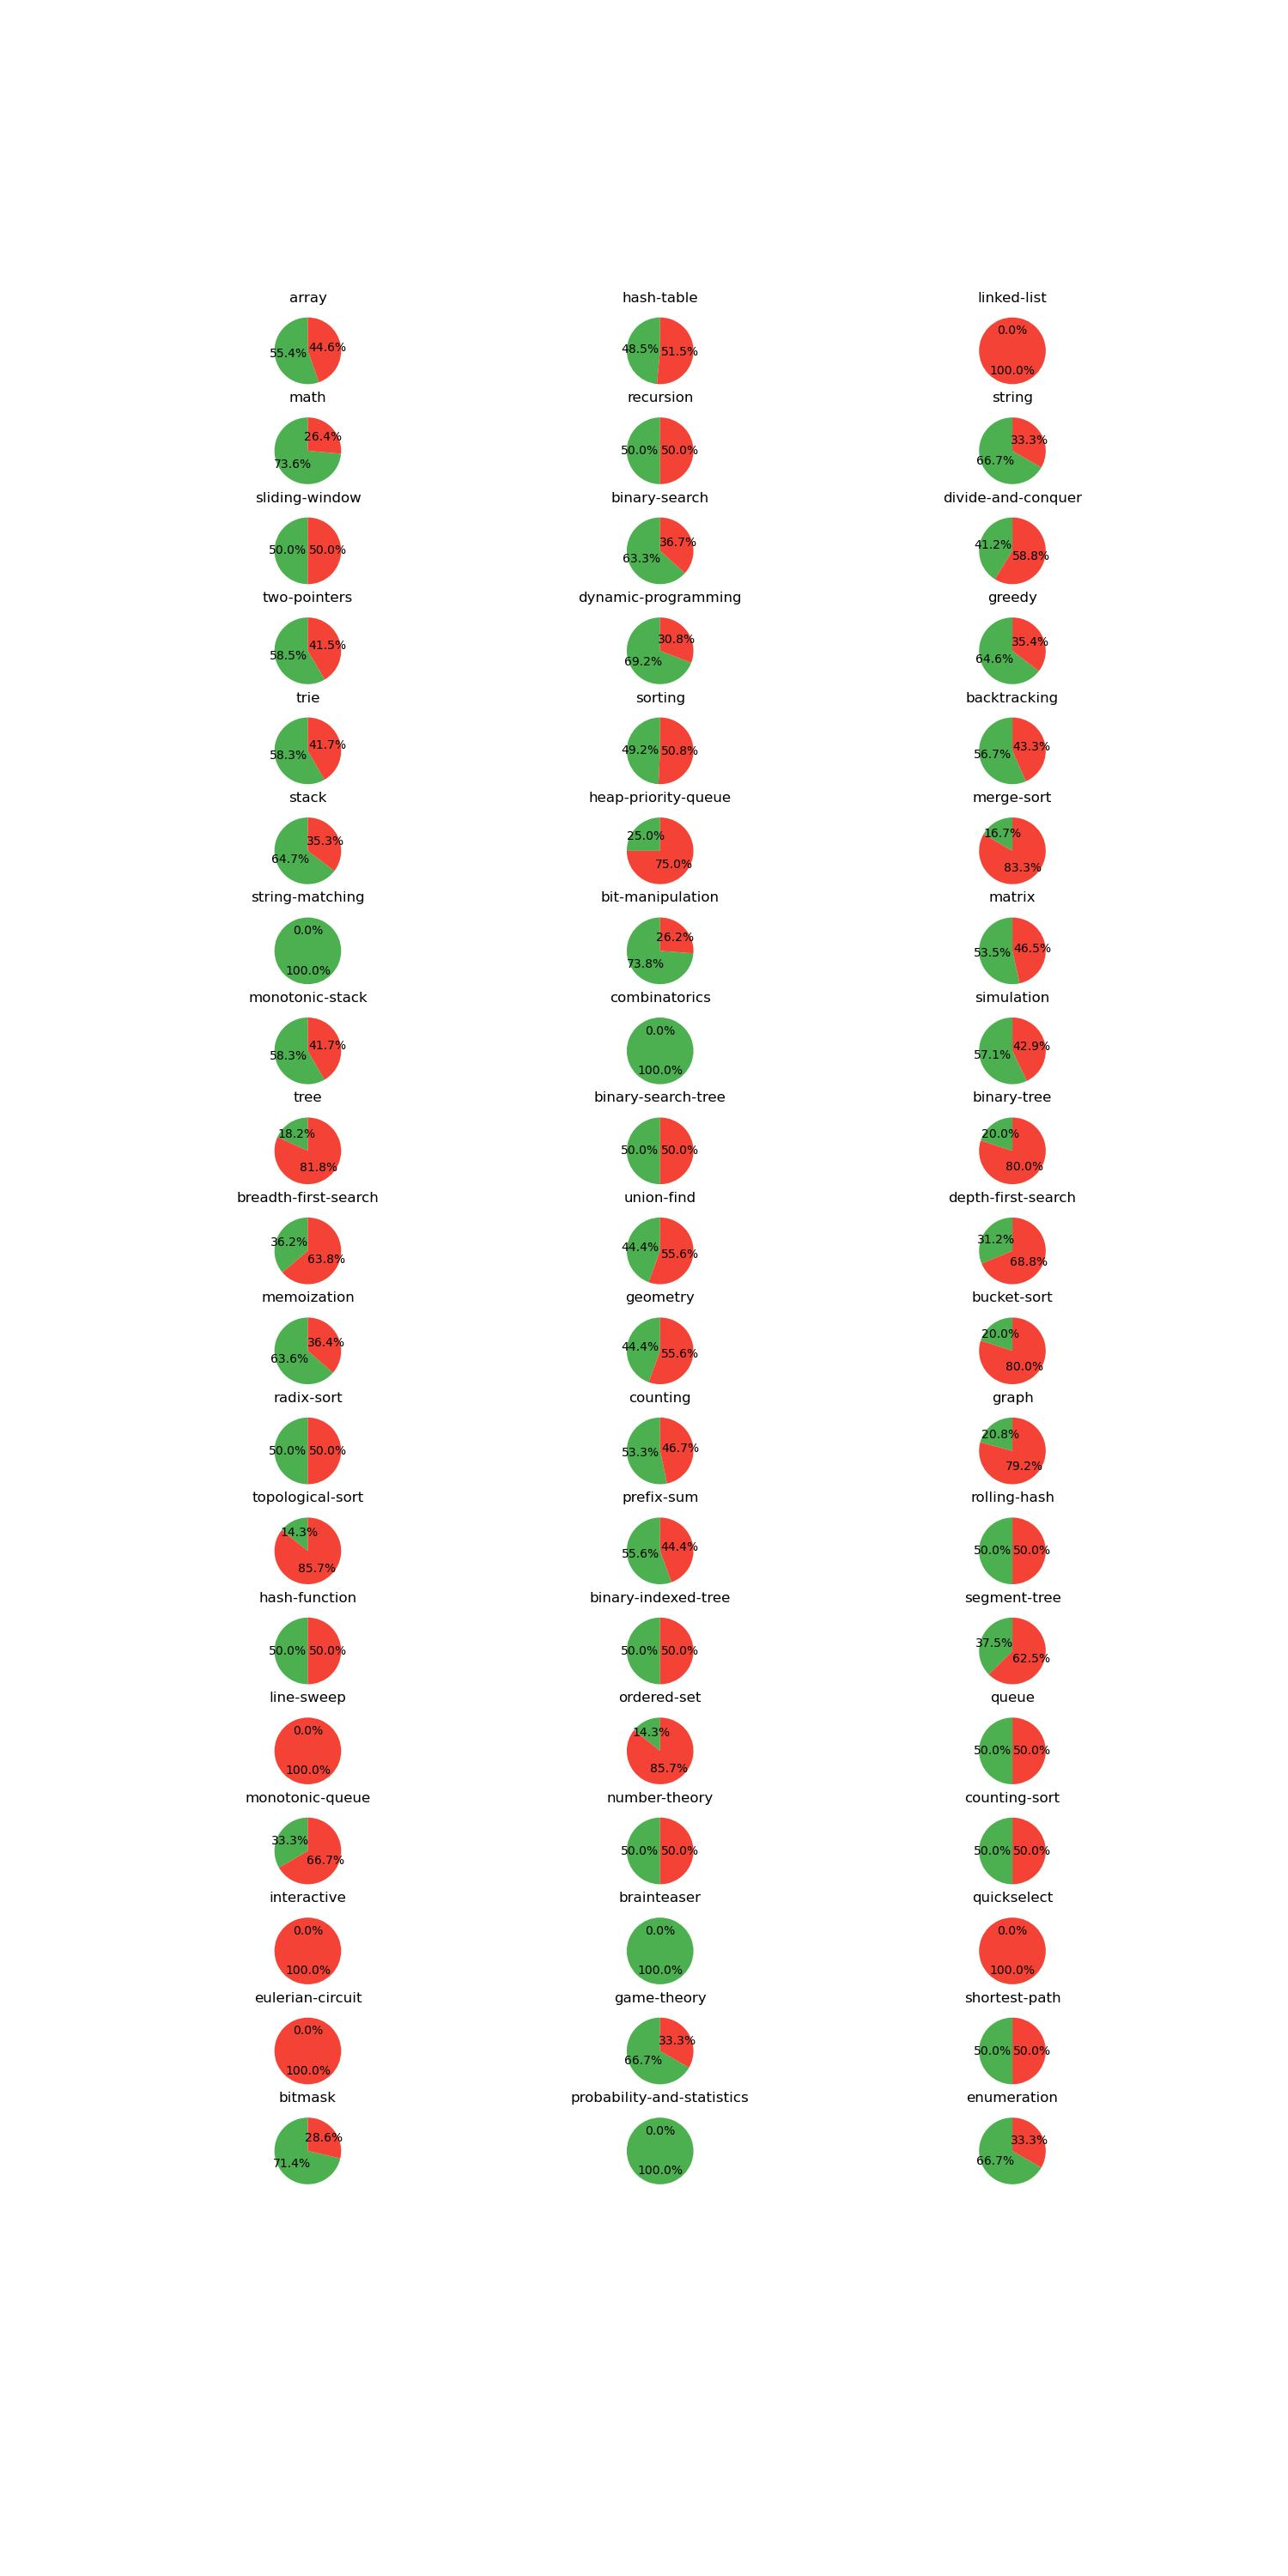
\includegraphics[width=0.75\textwidth, height=0.7\textheight]{figures/7/accepted_not_topicwise.jpg}
    \caption{Topic-wise acceptance rate for Prompt 7, illustrating the percentage of solutions accepted (green) and not accepted (red) across different undergraduate computer science topics.}
    \label{fig:topic_wise_acceptance_prompt_7}
\end{figure}

\begin{figure}[H]
    \centering
    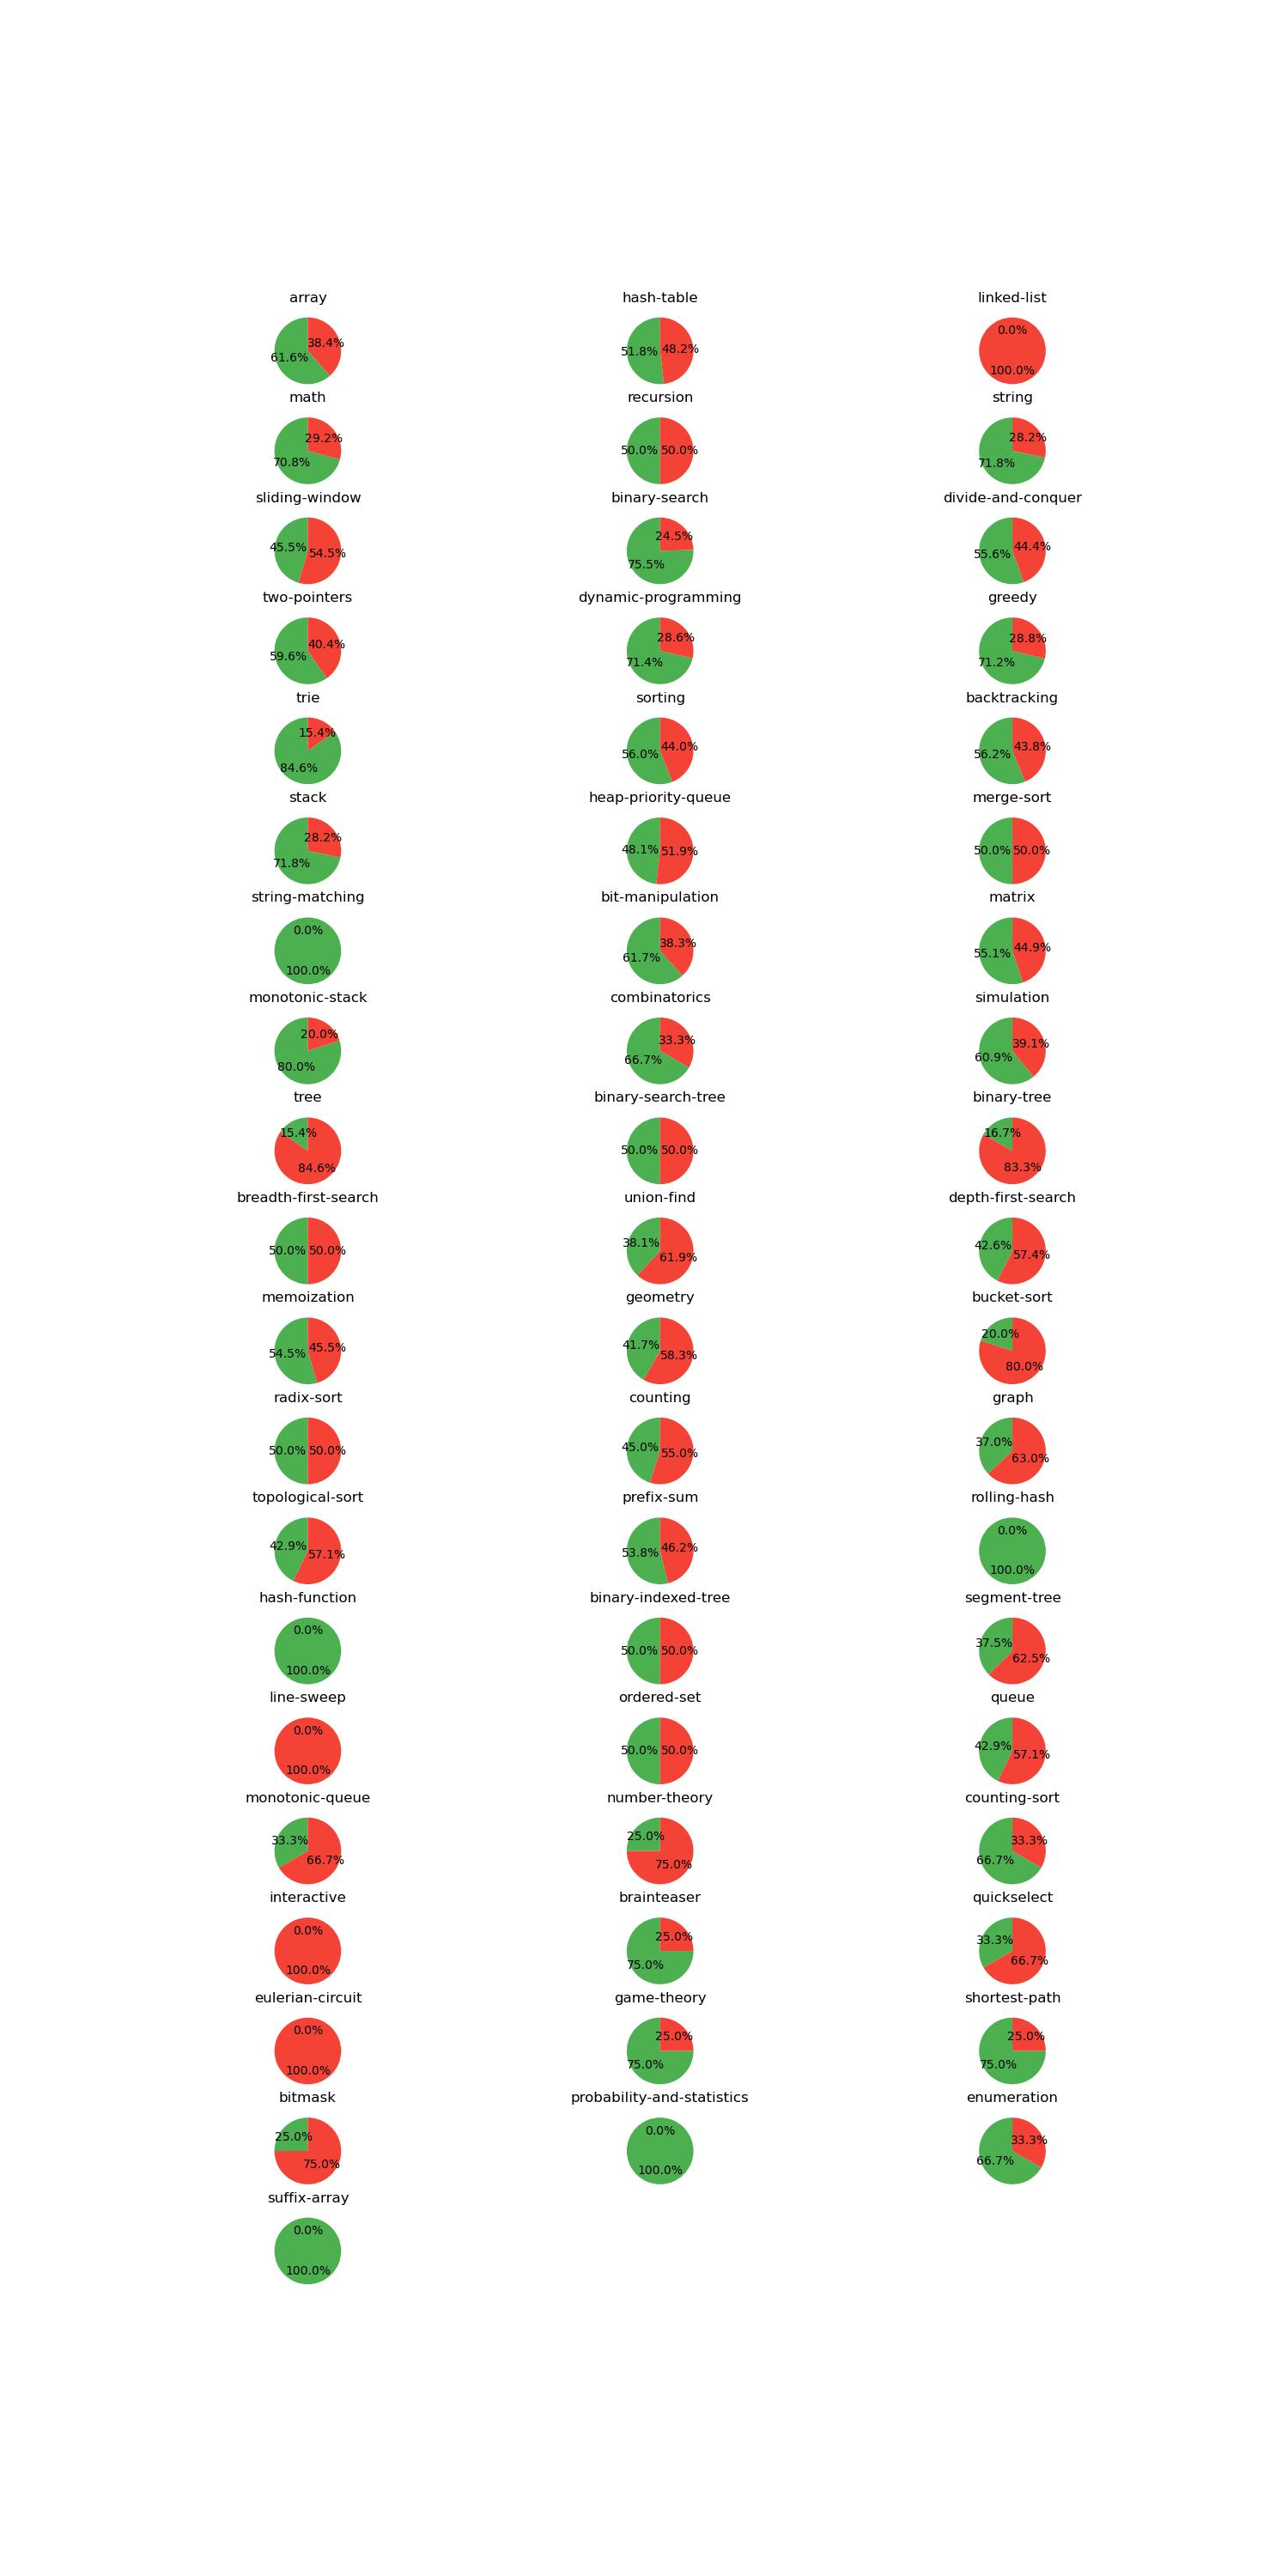
\includegraphics[width=0.75\textwidth, height=0.7\textheight]{figures/8/accepted_not_topicwise.jpg}
    \caption{Topic-wise acceptance rate for Prompt 8, illustrating the percentage of solutions accepted (green) and not accepted (red) across different undergraduate computer science topics.}
    \label{fig:topic_wise_acceptance_prompt_8}
\end{figure}

\begin{figure}[H]
    \centering
    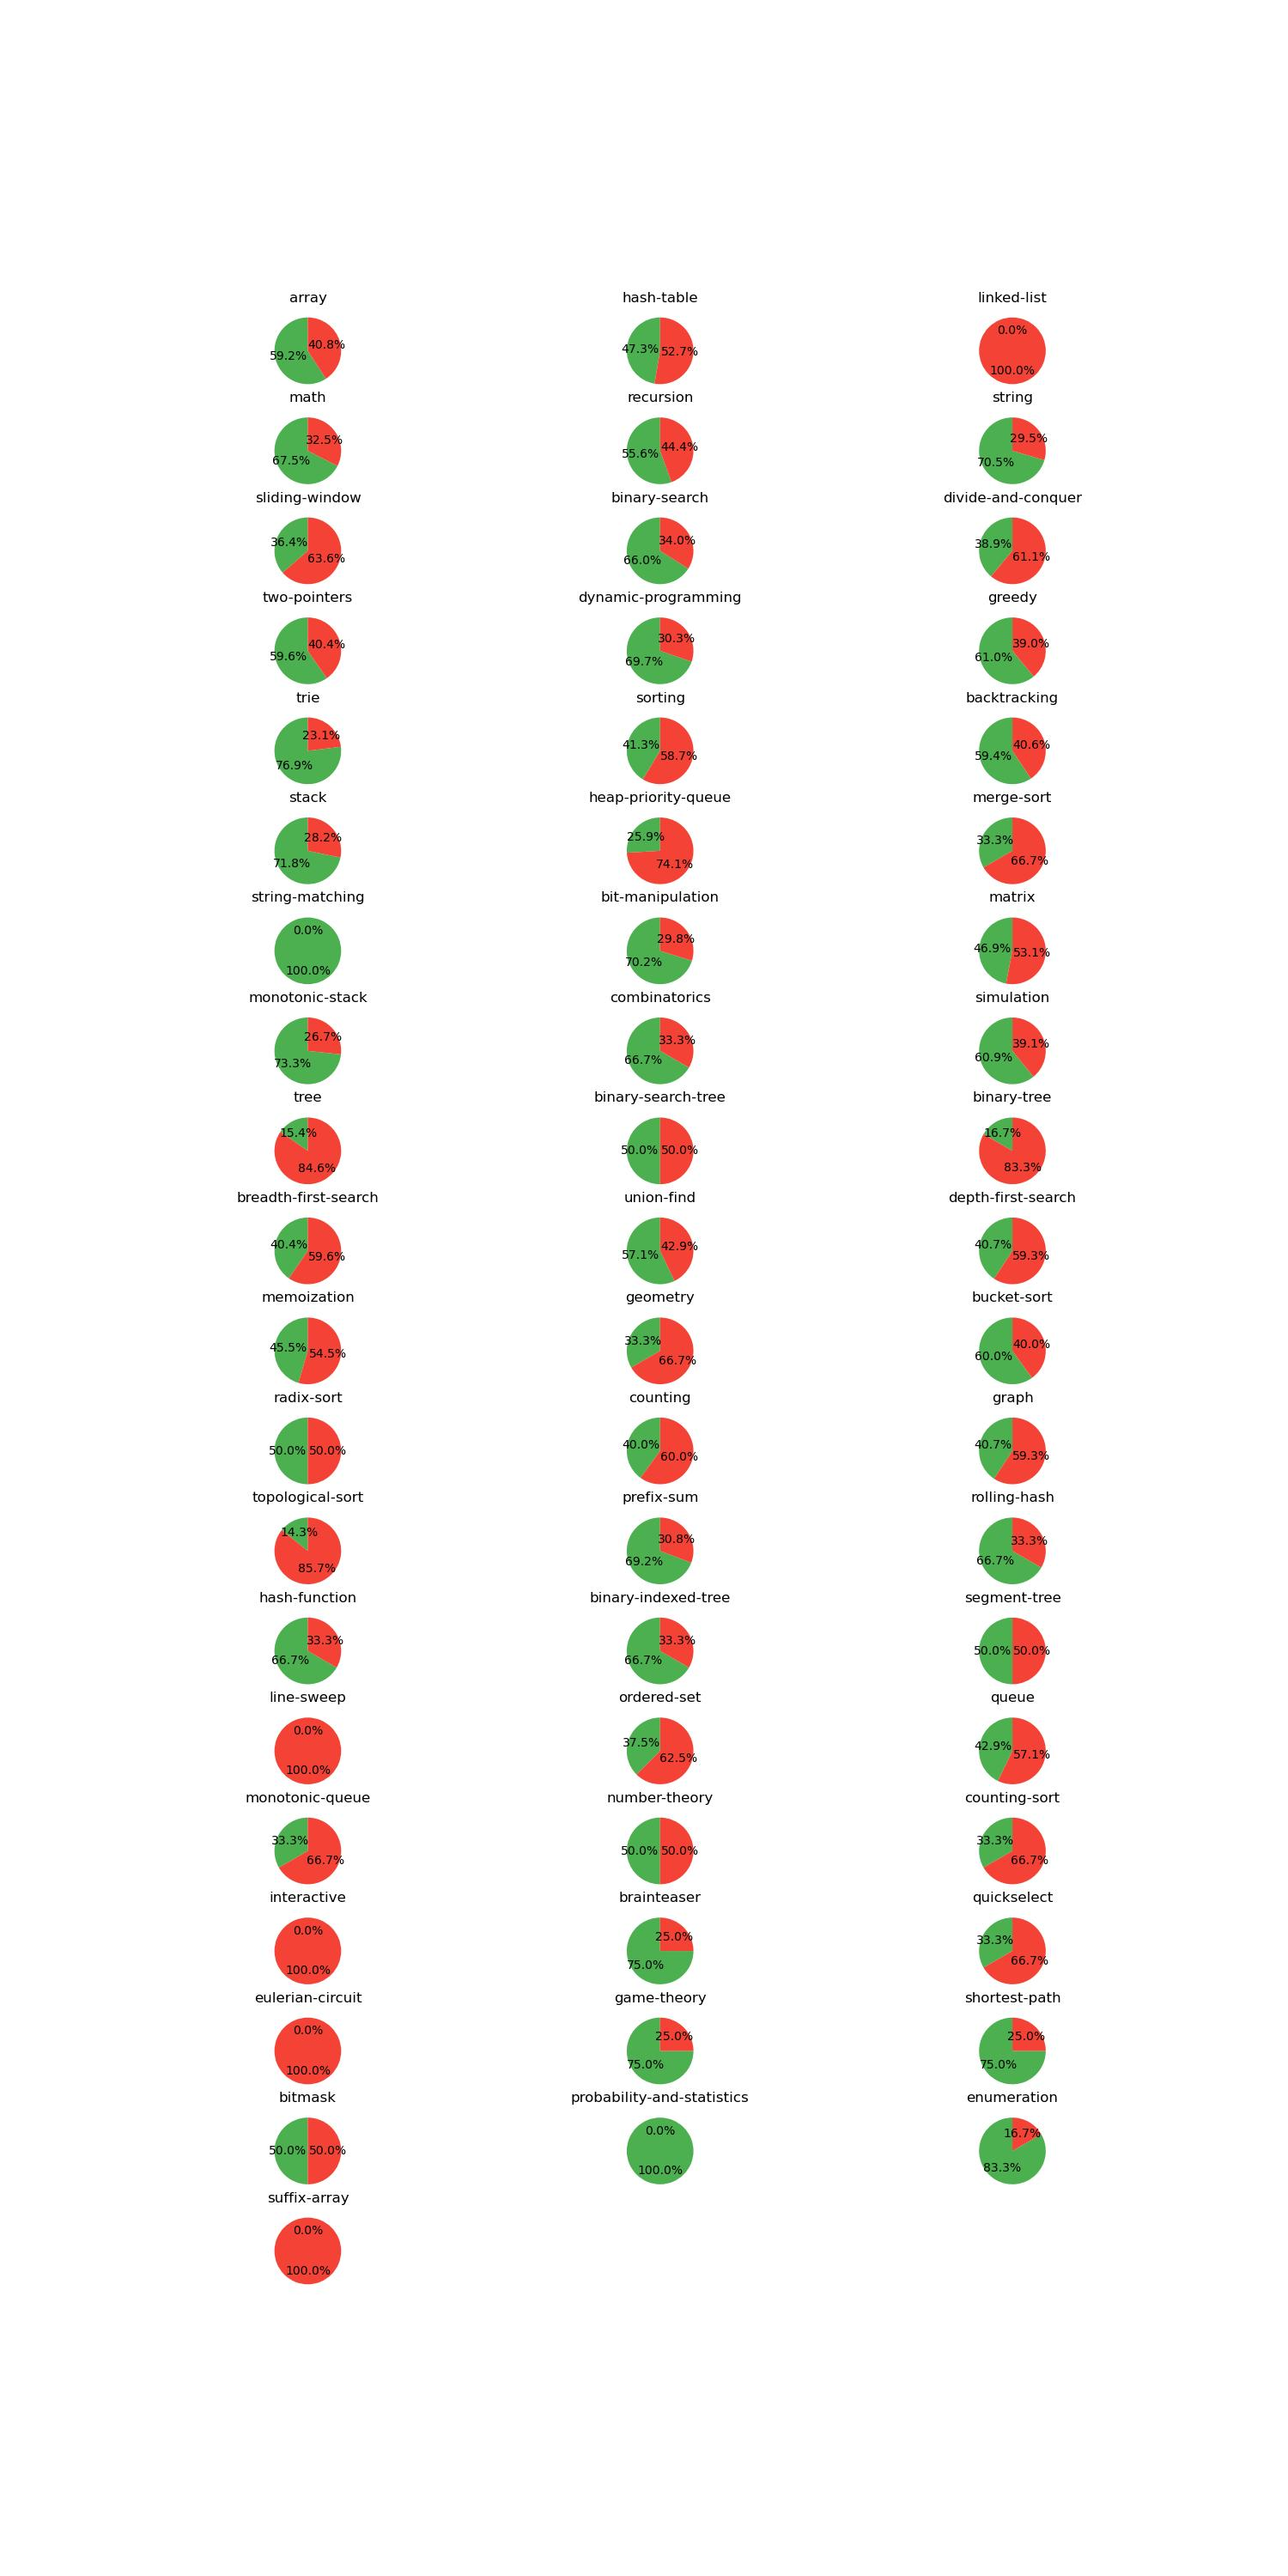
\includegraphics[width=0.75\textwidth, height=0.7\textheight]{figures/9/accepted_not_topicwise.jpg}
    \caption{Topic-wise acceptance rate for Prompt 9, illustrating the percentage of solutions accepted (green) and not accepted (red) across different undergraduate computer science topics.}
    \label{fig:topic_wise_acceptance_prompt_9}
\end{figure}

        \chapter{An Appendix Chapter (Optional)}
\label{appn:B}

...
    \end{appendices}
    
\end{document}
